\documentclass[oneside,a4paper]{article}

%%%%%%%%%%%%%%%%%%%%%%%%%%%%
\usepackage{amsthm}
\usepackage{amsmath}
\usepackage{amssymb}
%%%%%%%%%%%%%%%%%%%%%%%%%%%%%
\usepackage[greek,english]{babel}
\usepackage{alphabeta}
\usepackage[utf8]{inputenc}
\usepackage{mathtools}
\usepackage{blindtext}
\usepackage[T1]{fontenc}
\usepackage{titlesec}
\usepackage{sectsty}
\usepackage{verbatim}
\usepackage{multirow}
\chapternumberfont{\tiny} 
\chaptertitlefont{\Huge}
%ελληνικοι χαρακτηρες σε μαθ pdf utf-8
%%%%%%%%%%%%%%%%%%%%%%%%%%%%%%%%%
\usepackage{tikz-cd}
%\usepackage{hyperref}
\usepackage{xcolor}
\usepackage{framed}%frames
\usepackage{float}
\usepackage{array}
\usepackage{pbox}
\usepackage{caption}
%%%%%%%%%%%%%%%%%%%%%%%%
\usepackage{tikz}
%%%%%%%%%%%%%%%%%%%%%%%%%%
\usepackage{sagetex}
%%%%%%%%περιθώρια%%%%%%%%%%%%
\usepackage[a4paper,margin=3.5cm]{geometry}

\usepackage{graphicx,import}

\usepackage[n, % o r lambda
advantage,
operators,
sets,
adversary,
landau,
probability,
notions,
logic,
ff,
mm,
primitives,
events,
complexity,
oracles,
asymptotics,
keys ]{cryptocode}

\newtheorem*{theorem}{Θεώρημα}
\newtheorem*{lemma}{Λήμμα}
\newtheorem*{example}{Παράδειγμα}
\newtheorem*{defn}{Ορισμός}
\newtheorem*{prop}{Πρόταση}
\newtheorem{cor}{Πόρισμα}
\newtheorem*{remark}{Παρατήρηση}

\newcommand {\tl}{\textlatin}
%%%%%%%%%αριθμηση%%%%%%%%%%%%%%
\renewcommand{\theenumi}{\arabic{enumi}}
\renewcommand{\labelenumi}{{\rm(\theenumi)}}
\renewcommand{\labelenumii}{\roman{enumii}) }
%%%%%%%%%%%% New theorems %%%%%%%%%%%%%%%%%%%%%%%%

%%%%%%%%%%%%%%%%%%%%%%%%%%%%%%%%%%%%%%%%%%%%%%%%%%%
\newcommand{\Z}{\mathbb{Z}}
\newcommand{\Q}{\mathbb{Q}}
\newcommand{\Co}{\mathbb{C}}
\newcommand{\So}{\mathcal{S}}
\newcommand{\C}{\mathcal{C}}

\newcommand{\Sheaf}{(\So, \pi, X)}
\usepackage{listings}
\usepackage{color}

\newcommand{\el}{\lambda}
\newcommand{\eL}{\Lambda}
\newcommand{\presheaf}{(S(U),\rho^U_V)_{V\subseteq U\in \tau_X}}
\newcommand{\ds}{(A_{\lambda},\phi^{\lambda_1}_{\lambda_2})}
\newcommand{\dsb}{(B_{\lambda},\psi^{\lambda_1}_{\lambda_2})}
\newcommand{\dlimit}{(A,\phi_{\lambda})}
\newcommand{\openx}{\mathcal{N}^0_x}

\newcommand{\curly}{\mathrel{\leadsto}}

\newcommand{\defeq}{\mathrel{\stackrel{\makebox[0pt]{\mbox{\normalfont\tiny \text{ορσ}}}}{=}}}

\newcommand{\incfig}[1]{%
    \fontsize{12pt}{12pt}\selectfont %χρησιμοποιώ height 600 width 300 pixels
    \def\svgwidth{2in}
    \import{./figures/}{#1.pdf_tex}
}

\begin{document}
	
	
	\selectlanguage{greek}
	%\pagenumbering{roman}
	
	
	\begin{framed}	
		%\vspace{0.3truecm}
		\begin{center}
			\huge Κρυπτογραφία Ελλειπτικών Καμπυλών
		\end{center}
		%\vspace{0.3truecm}
		\begin{center}
            Ειδικά Θέματα: Κρυπτογραφία
		\end{center}
		\vspace{0.3truecm}
		\begin{center}
            Νούλας Δημήτριος\\
            ΑΜ: 7112112100016\\
            \tl{dnoulas@math.uoa.gr}
\end{center}
		\vspace{0.3truecm}
	\end{framed}
	\vspace*{\fill}
	\begin{center}
	\includegraphics[width=0.5\textwidth]{C:/Users/dimit/Desktop/TeX/uoa_logo}
	%\includegraphics[width=0.5\textwidth]{/mnt/c/Users/dimit/Desktop/TeX/uoa_logo}
	\end{center}
\vspace{1cm}
\pagebreak

\tableofcontents
\pagebreak

\section{Εισαγωγή}
Οι ελλειπτικές καμπύλες οφείλουν το όνομά τους στο πρόβλημα της εύρεσης μήκους τόξου πάνω σε ελλείψεις. Ουσιαστικά, το πρόβλημα αυτό ανάγεται στον υπολογισμό των λεγόμενων ελλειπτικών ολοκληρωμάτων που έχουν την μορφή:

$$\int \frac{1}{\sqrt{x^2 + ax + b}} dx$$

\noindent Ο υπολογισμός των παραπάνω ολοκληρωμάτων ήταν ένα από τα κύρια προβλήματα της ανάλυσης στους προηγούμενους αιώνες και διάσημοι μαθηματικοί όπως οι \tl{Euler, Weierstrass, Abel, Jacobi} ασχολήθηκαν σε αυτόν τον τομέα. Το παραπάνω ολοκλήρωμα οδηγεί στην μελέτη δύο μιγαδικών συναρτήσεων $x,y$ που ικανοποιούν μια εξίσωση της μορφής:
$$y^2 = x^3 + ax + b$$ ή ισοδύναμα στην μελέτη των μιγαδικών αριθμών $(x,y) \in \mathbb{C}^2$ που ικανοποιούν την παραπάνω εξίσωση. Η σύγχρονη μελέτη αυτού του προβλήματος εντάσσεται στα πλαίσια της μελέτης των επιφανειών \tl{Riemann} στην γεωμετρία. Στα πλαίσια της κρυπτογραφίας και γενικότερα της επιστήμης των υπολογιστών, αυτές οι εξισώσεις έχουν ιδιαίτερο ενδιαφέρον όταν αντί για το $\mathbb{C}$, έχοντας κατά νου ότι η μνήμη ενός υπολογιστή είναι πεπερασμένη, τις κοιτάμε πάνω από τα πεπερασμένα σώματα $\mathbb{F}_q$. Δίνουμε τώρα τον ορισμό μιας ελλειπτικής καμπύλης.

\vspace*{0.1cm}
\begin{defn}[Ελλειπτική Καμπύλη]
	Έστω $x^3 +ax + b$ ένα κυβικό πολυώνυμο υπέρ ενός σώματος $K$ το οποίο έχει απλές ρίζες. Μια ελλειπτική καμπύλη υπέρ του σώματος $K$ θα είναι το σύνολο των σημείων $x,y \in K$ που ικανοποιούν την εξίσωση:
	$$E: \quad y^2 = x^3 + ax + b$$ μαζί με ένα σημείο $\mathcal{O}$ στο άπειρο. Η συνθήκη για τις απλές ρίζες είναι ισοδύναμη με την σχέση $\Delta = 16(4a^3 +27b^2)\neq 0$.
\end{defn}

$ $\newline
Χωρίς να είναι ακόμα ξεκάθαρο τι είναι το σημείο στο άπειρο, είναι χρήσιμο να βλέπουμε τις ελλειπτικές καμπύλες σε έναν ευρύτερο χώρο, το λεγόμενο προβολικό επίπεδο, το οποίο επιταχύνει τους υπολογισμούς και μπορούμε εύκολα να αναπαριστούμε τα σημεία της ελλειπτικής καμπύλης σαν λίστες $[x:y:z]$. Δίνουμε τον εξή ορισμό:

%https://crypto.stackexchange.com/questions/40947/what-is-the-projective-space
\vspace*{0.1cm}
\begin{defn}[Προβολικό Επίπεδο]
	Έστω $K$ σώμα και στο σύνολο των διατεταγμένων τριάδων $K^3 - (0,0,0)$ ορίζουμε την σχέση ισοδυναμίας $(x_1,y_1,z_1) \sim (x_2,y_2,z_2)$ αν και μόνο αν υπάρχει $\lambda \in K^*$ με $(x_1,y_1,z_1) = \lambda (x_2,y_2,z_2)$. Το σύνολο πηλίκο το ονομάζουμε {\em προβολικό επίπεδο} και στην βιβλιογραφία συμβολίζεται με
	$$\mathbb{P}^2(K) = \frac{K^3 - (0,0,0)}{\sim }$$
\end{defn}

$ $\newline
Ουσιαστικά, βλέπουμε τις ευθείες σαν ένα στοιχείο του χώρου, αφού όλα τα σημεία που βρίσκονται πάνω σε μια ευθεία που περνάει από το $(0,0,0)$ είναι ισοδύναμα ως προς την σχέση $\sim$. Θα συμβολίζουμε την κλάση ισοδυναμίας ενός σημείου $(x,y,z)\neq (0,0,0)$ ως $[x:y:z]$. Παρατηρούμε ότι τα σημεία $[x:y:1]$ είναι σε ένα προς ένα και επί αντιστοιχία με το επίπεδο $K^2$, ενώ τα σημεία $[x:y:0]$ αποτελούν μια ευθεία που την ονομάζουμε ευθεία στο άπειρο. Μπορούμε να χωρίσουμε το προβολικό επίπεδο στα στοιχεία που έχουν αντιπρόσωπο $z=0$ και σε αυτά που δεν έχουν, δηλαδή στις ευθείες που περνάνε από το $(0,0,0)$ στο επίπεδο $\{x,y,0\}$ και σε αυτές που δεν ζουν μέσα σε αυτό. Από τους ορισμούς, η δεύτερη κατηγορία θα τέμνει το επίπεδο $z=1$ και άρα κάθε τέτοιο στοιχείο στο προβολικό επίπεδο θα έχει αντιπρόσωπο $[x:y:1]$. Με την ίδια λογική, οι ευθείες για τις οποίες ισχύει $z=0$ θα έχουν αντιπρόσωπο $[x:1:0]$, εκτός από αυτές που είναι παράλληλες στο επίπεδο $\{y=1,z=0\}$ που είναι ο άξονας των $x$, δηλαδή στα σημεία $[x:0:0]$. Συνοπτικά, τα στοιχεία του προβολικού επιπέδου έχουν τρία είδη αντιπροσώπων:

$$[1:0:0], \quad [x:1:0], \quad [x:y:0]$$ 


\vspace*{0.1cm}
\noindent Για κάθε πολυώνυμο $f(x,y) \in K[x,y]$ βαθμού $n$:
$$f(x,y) = \sum\limits_{i,j} a_{ij}x^i y^j$$ θα συμβολίζουμε με $F$ το ομογενές πολυώνυμο:
$$F(x,y,z) = \sum\limits_{i,j} a_{ij}x^i y^j z^{n-i-j}$$ και αυτήν την διαδικασία την ονομάζουμε ομογενοποίηση.

$ $\newline
Επιστρέφοντας στις ελλειπτικές καμπύλες, το να τις δούμε μέσα στο προβολικό επίπεδο είναι ισοδύναμο με το να ψάχνουμε στοιχεία $[x:y:z]$ που ικανοποιούν την ομογενοποιημένη εξίσωση:
$$E: \quad zy^2 =  x^3 + axz^2 + bz^3$$

$ $\newline
Βλέπουμε ότι το στοιχείο $[1:0:0]$ δεν ανήκει πάνω στην καμπύλη, ενώ τα στοιχεία με $z=1$ μας επιστρέφουν την αρχική εξίσωση $y^2 = x^3 + ax +b$ της ελλειπτικής καμπύλης. Για τα στοιχεία με $z=0$ έχουμε ότι:
$$z= 0 \implies 0 = y^2z = x^3 + axz^2 + bz^3 = x^3$$ δηλαδή $x=0$ και άρα τα σημεία που βρίσκονται πάνω στην ελλειπτική με $z=0$ είναι αυτά πάνω στον $y$-άξονα, τα οποία όλα ανήκουν στην κλάση $\mathcal{O} = [0:1:0]$. Αυτό είναι το στοιχείο που δεν μπορούμε να προσδιορίσουμε με την αρχική εξίσωση της ελλειπτικής καμπύλης, το λεγόμενο σημείο στο άπειρο.

$ $\newline
Αξίζει να σημειώσουμε ότι για μια ελλειπτική καμπύλη υπάρχει και η πιο γενική εξίσωση του \tl{Weierstrass}:
$$y^2 +a_1 xy + a_3 y = x^3 +a_2 x^2 + a_4 x + a_6$$ η οποία είναι ισοδύναμη με την αρχική κάνοντας μια γραμμική αλλαγή μεταβλητής. Για να έχουμε μια εικόνα, δύο ελλειπτικές καμπύλες πάνω από τους ρητούς έχουν γραφική παράσταση όπως φαίνεται στην επόμενη σελίδα:
\begin{center}
	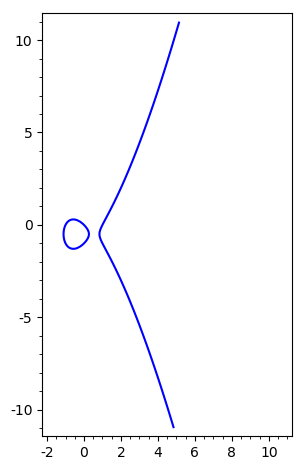
\includegraphics[width=0.5\textwidth]{C:/Users/dimit/Desktop/TeX/EC/ec1_pic}
	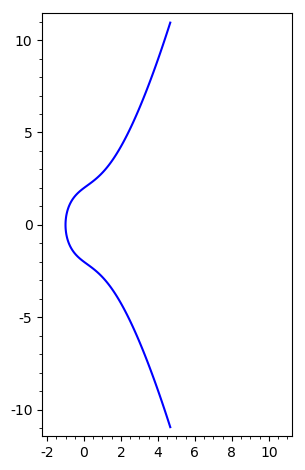
\includegraphics[width=0.5\textwidth]{C:/Users/dimit/Desktop/TeX/EC/ec2_pic}
	%\includegraphics[width=0.5\textwidth]{/mnt/c/Users/dimit/Desktop/TeX/uoa_logo}
\end{center}
\pagebreak
\noindent Τις οποίες παράγουμε ως εξής:
%\begin{center}
	%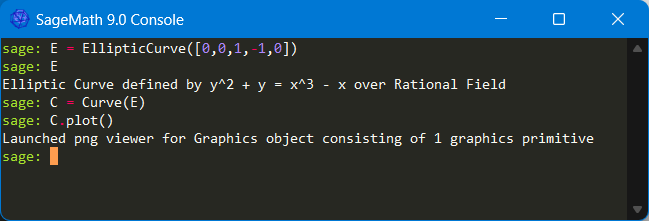
\includegraphics[width=0.5\textwidth]{C:/Users/dimit/Desktop/TeX/EC/ec1_code}
	%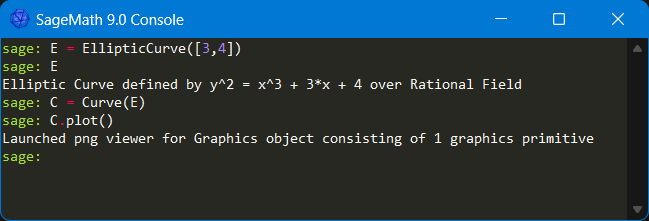
\includegraphics[width=0.5\textwidth]{C:/Users/dimit/Desktop/TeX/EC/ec2_code}
	%\includegraphics[width=0.5\textwidth]{/mnt/c/Users/dimit/Desktop/TeX/uoa_logo}
%\end{center}
%ec1
%ec2


\begin{center}
\selectlanguage{english}
\begin{sageblock}
	sage: E1 = EllipticCurve([0,0,1,-1,0])
	sage: E1
	Elliptic Curve defined by y^2 + y = x^3 -x over Rational Field
	sage: E2 = Elliptic Curve([3,4])
	sage: E2
	Elliptic curve defined by y^2 = x^3 + 3*x + 4 over Rational Field
	sage: C1 = Curve(E1)
	sage: C2 = Curve(E2)
	sage: C1.plot()
	sage: C2.plot()
\end{sageblock}
\end{center}

\noindent Ενώ στο προβολικό επίπεδο:

%proj1
\begin{center}
	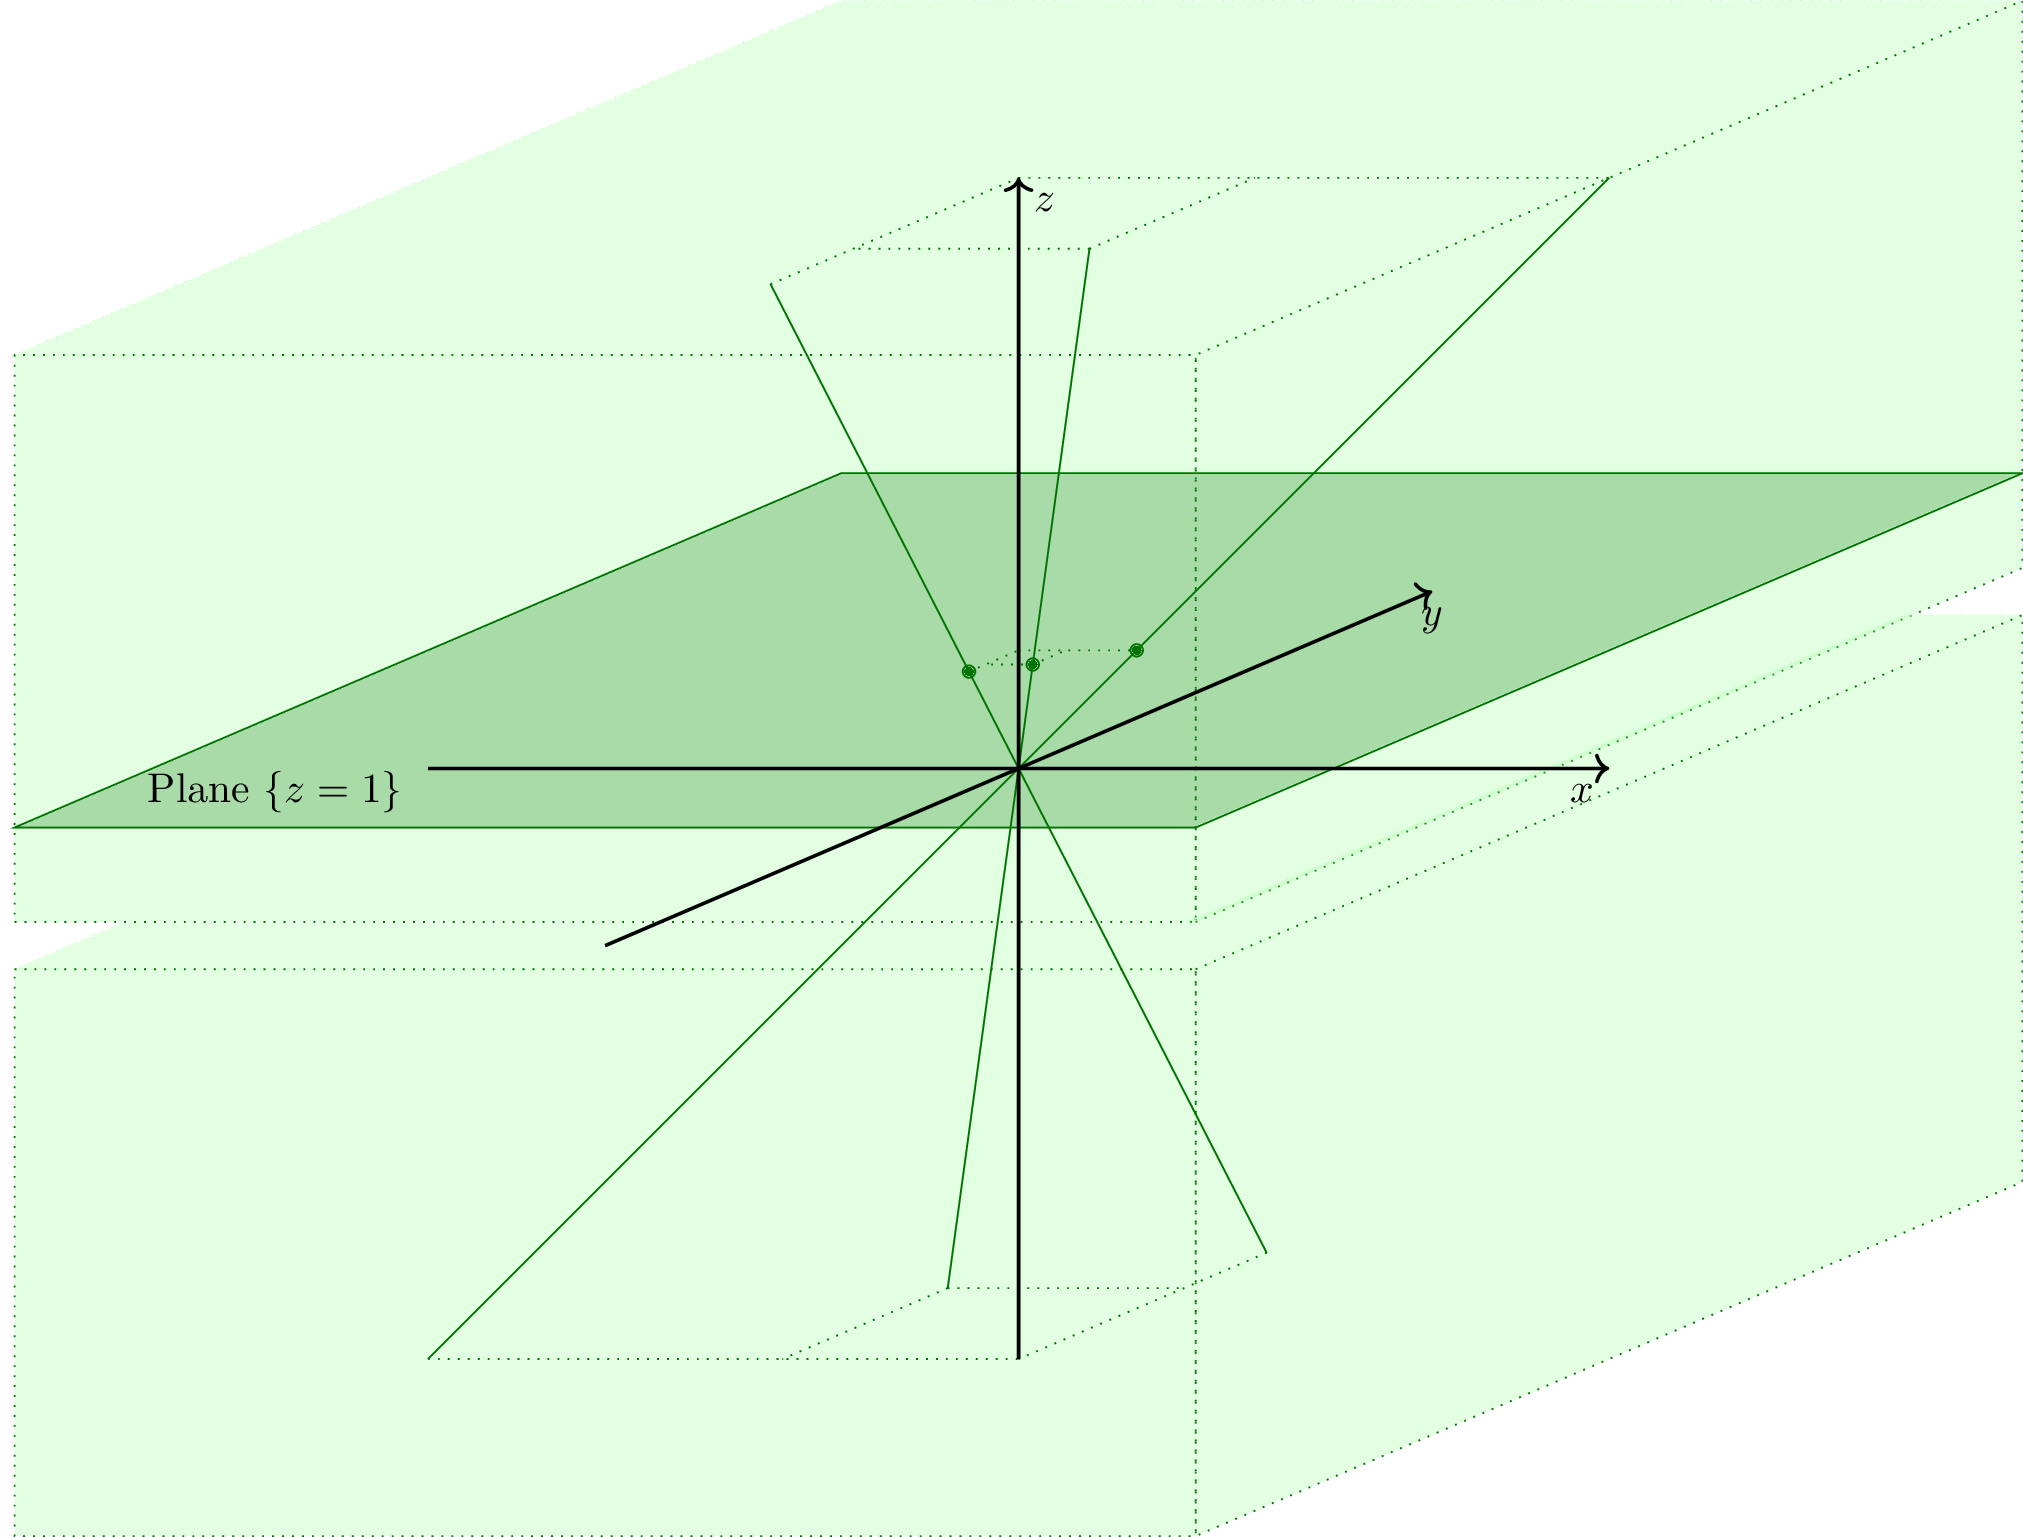
\includegraphics[width=0.5\textwidth]{C:/Users/dimit/Desktop/TeX/EC/proj1}
\end{center}

\noindent Μια ελλειπτική καμπύλη φαίνεται ως:

%proj2
\begin{figure}[H]
	\centering
	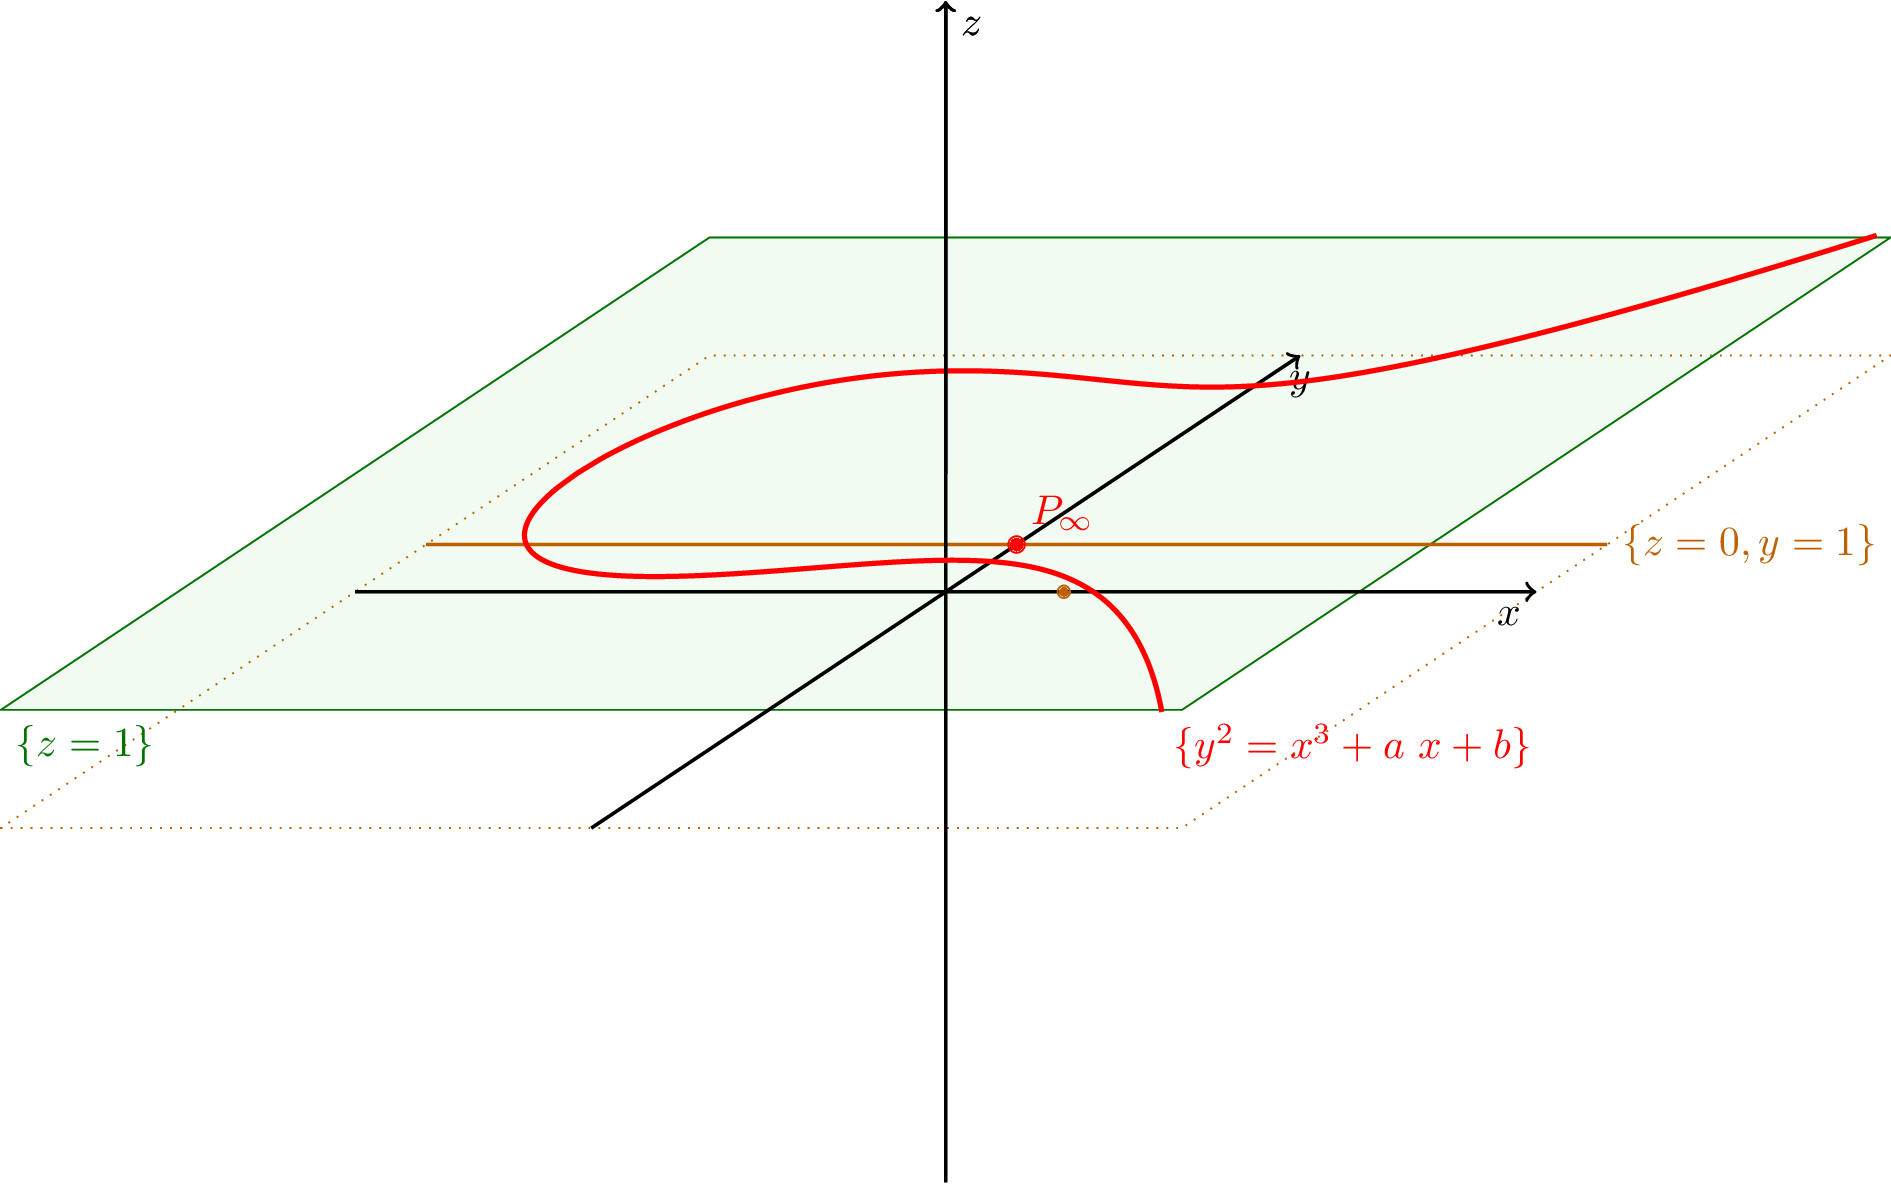
\includegraphics[width=0.5\textwidth]{C:/Users/dimit/Desktop/TeX/EC/proj2}
	\captionsetup{labelformat=empty}
	\caption{Οι εικόνες είναι από την πηγή: \tl{crypto.stackexchange.com/questions/40947/what-is-the-projective-space}}.
\end{figure}
%Οι εικόνες είναι από τον σύνδεσμο: \href{https://crypto.stackexchange.com/questions/40947/what-is-the-projective-space}{\tl{what is the projective space}}.

%εικόνες από link 
%https://crypto.stackexchange.com/questions/40947/what-is-the-projective-space
$ $\newline
Στα πεπερασμένα σώματα που μας ενδιαφέρει στην πράξη, η ελλειπτική καμπύλη έχει γραφική παράσταση σαν την παρακάτω. Εφόσον έχουμε στο σώμα χαρακτηριστική $p>0$ πρώτο αριθμό, παίρνουμε τα σημεία $(x,y)$ που ικανοποιούν την σχέση:
$$y^2 \equiv x^3 + ax + b \ \mod p$$
\selectlanguage{english}
\begin{sageblock}
	sage: E = EllipticCurve(FiniteField(101),[3,4])
	sage: P = plot(E,rgbcolor=(0,0,1))
\end{sageblock}

%ec_finite
\begin{figure}[H]
	\centering
	\captionsetup{labelformat=empty}
	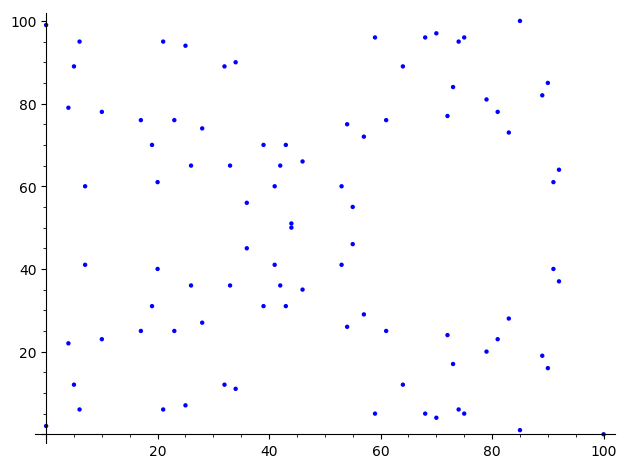
\includegraphics[width=0.8\textwidth]{C:/Users/dimit/Desktop/TeX/EC/ec_finite}
	\caption{Η ελλειπτική καμπύλη $y^2 = x^3 +3x + 4$ πάνω από το σώμα $\mathbb{F}_{101}$.}
\end{figure}

$ $\newline
Στην συνέχεια, θα ορίσουμε τον τρόπο πρόσθεσης δύο σημείων πάνω στην ελλειπτική καμπύλη και θα δώσουμε το θεώρημα το οποίο μας επιτρέπει να κάνουμε κρυπτογραφία πάνω σε ελλειπτικές καμπύλες. Έστω $P=(x_1,y_1)$ και $Q = (x_2,y_2)$ δύο σημεία επί της ελλειπτικής καμπύλης. Σχηματίζουμε την ευθεία που ενώνει τα δύο σημεία. Αυτή η ευθεία τέμνει την ευθεία σε ένα τρίτο σημείο $PQ$. Από το σημείο $PQ$ φέρνουμε την κάθετη στον άξονα των $x$. To σημείο τομής της κάθετης με την ελλειπτική καμπύλη το ορίζουμε ως $P+Q$, δηλαδή ως άθροισμα των σημείων $P, Q$. Στην περίπτωση που θέλουμε να υπολογίσουμε το σημείο $P+P$ θεωρούμε την εφαπτομένη πάνω στο $P$, αντί για την χορδή όπως στην προηγούμενη περίπτωση. Όταν ένας προσθετέος είναι το $\mathcal{O}$ έχουμε ότι $P+\mathcal{O} = P$, δηλαδή το $\mathcal{O}$ δρα ως ουδέτερο σημείο στην πρόσθεση.

$ $\newline
Για να εκφράσουμε αλγεβρικά τους τύπους πρόσθεσης για τα σημεία $P =  (x_1,y_1)$ και $Q= (x_2,y_2)$, υποθέτουμε ότι $P,Q \neq \mathcal{O}$ και αν $x_1 = x_2$ και $y_1 = -y_2$ τότε $P+Q = \mathcal{O}$, δηλαδή συμμετρικά σημεία ως προς τον άξονα $x$ έχουν άθορισμα $\mathcal{O}$. Διαφορετικά θέτουμε:

$$\lambda = 
\begin{cases}\frac{3x_1 + a }{2y_1}, & \text{ αν } P = Q \\
\frac{y_1 -y_2}{x_1 - x_2}, & \text{ αν } P \neq Q \end{cases}$$
και βασιζόμενοι στο $\lambda$ το σημείο $P+Q$ έχει συντεταγμένες:

$$P+Q = (\lambda^2 -x_1 -x_2, \ \lambda(x_1- x_2) -y_1)$$
%σχηματικά, ο τρόπος που προσθέτουμε τα σημεία είναι ως εξής:
%pic wikipedia addition

%\begin{figure}[H]
	%\centering
	%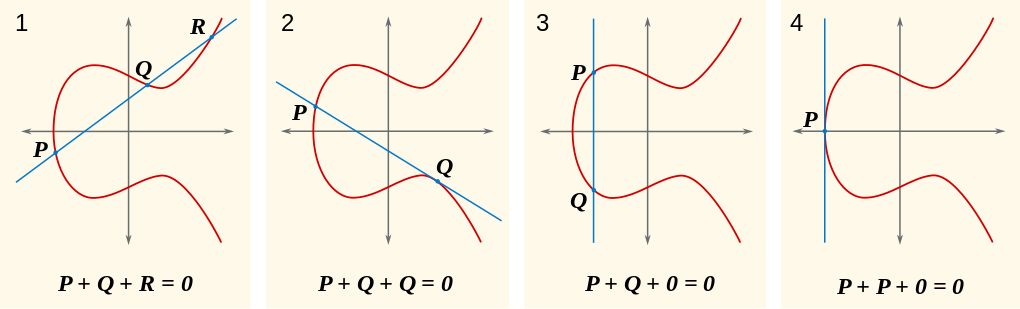
\includegraphics[width=0.8\textwidth]{C:/Users/dimit/Desktop/TeX/EC/addition_law}
%\end{figure} 
%δεν έχω 'σχηματικά' αλλά ιδιότητες addition τριών σημείων που κάνουν 0

$ $\newline
Για να ορίσουμε βαθμωτό πολλαπλασιασμό των σημείων της ελλειπτικής καμπύλης χρησιμοποιούμε τον κανόνα της πρόσθεσης, δηλαδή:
$$n \cdot P = P + P + \cdots + P$$

$ $\newline
Το θεώρημα στο οποίο βασιζόμαστε έιναι το εξής:

\begin{theorem} Τα σημεία της ελλειπτικής καμπύλης με πράξη την πρόσθεση που ορίστηκε και ουδέτερο στοιχείο το $\mathcal{O}$ αποτελούν αβελιανή ομάδα.
\end{theorem}

$ $\newline
Όλα τα παραπάνω μπορούν να υλοποιηθούν απλά με την γλώσσα προγραμματισμού \tl{Python} ως εξής:

\vspace*{0.1cm}
\selectlanguage{english}
\begin{lstlisting}[language = Python]
from Crypto.Util.number import inverse

def point_add(p, q, E):
    zero = (0, 0)
    if p == zero:
        return q
    elif q == zero:
        return p
    else:
        x1, y1 = p
        x2, y2 = q
        if x1 == x2 and y1 == -y2:
            return zero

        Ea, Ep = E['a'], E['p']
        if p != q:
            lmd = (y2 - y1) * inverse(x2 - x1, Ep)
        else:
            lmd = (3 * (x1**2) + Ea) * inverse(2 * y1, Ep)
        x3 = ((lmd**2) - x1 - x2) % Ep
        y3 = (lmd * (x1 - x3) - y1) % Ep
        return x3, y3


def scalar_mult(n, p, E):
    q, r = p, (0, 0)
    while n > 0:
        if n % 2 == 1:
            r = point_add(r, q, E)
        q = point_add(q, q, E)
        n //= 2
    return r

\end{lstlisting}

Ώστόσο, δεν χρειάζεται κανείς να ξεκινήσει από το μηδέν. Για τους μαθηματικούς είναι αρκετά χρήσιμο το πακέτο \tl{SageMath} βασιζόμενο στην γλώσσα προγραμματισμού \tl{Python} που κάνει τους υπολογισμούς στο προβολικό επίπεδο:
\pagebreak
\selectlanguage{english}
\begin{sageblock}
	sage: E = EllipticCurve(FiniteField(101),[3,4])
	sage: P = E.point([0,2])
	sage: P
	(0:2:1)
	sage: P.order()
	23
	sage: for i in range(1,P.order()+1):
	....: 	i*P
	....:
	(0 : 2 : 1)
	(70 : 97 : 1)
	(55 : 46 : 1)
	(83 : 73 : 1)
	(32 : 12 : 1)
	(4 : 22 : 1)
	(21 : 95 : 1)
	(79 : 81 : 1)
	(23 : 76 : 1)
	(20 : 61 : 1)
	(44 : 50 : 1)
	(44 : 51 : 1)
	(20 : 40 : 1)
	(23 : 25 : 1)
	(79 : 20 : 1)
	(21 : 6 : 1)
	(4 : 79 : 1)
	(32 : 89 : 1)
	(83 : 28 : 1)
	(55 : 55 : 1)
	(70 : 4 : 1)
	(0 : 99 : 1)
	(0 : 1 : 0)
\end{sageblock}

$ $\newline
Επιπλέον, υπάρχει και η βιβλιοθήκη \tl{PyCryptodome} της \tl{Python} που υποστηρίζει ολόκληρο το \tl{Public Key Infrastructure} και στο επόμενο παράδειγμα φαίνεται πώς μπορούμε να επιλέξουμε μια ελλειπτική καμπύλη, να δημιουργήσουμε ιδιωτικό και δημόσιο κλειδί και να τα χειριστούμε σε αρχεία:

\selectlanguage{english}
\begin{lstlisting}[language = Python]
	from Crypto.PublicKey import ECC

	private_key = ECC.generate(curve='P-256')
	public_key = private_key.public_key()
	print(public_key)
	%EccKey(curve='NIST P-256', point_x=7656170542301456206
	1860150560615631451455188074817536478296461957767192909
	320,
	point_y=69089698564456934829353568825198745013281366555
	012989239449323649065476753678)

	f = open('myprivatekey.pem','wt')
	f.write(key.export_key(format='PEM'))
	f.close()

	f = open('myprivatekey.pem','rt')
	key = ECC.import_key(f.read())
\end{lstlisting}


$ $\newline
Πριν κλείσει το κεφάλαιο αξίζει να αναφερθούμε σε κάποια κομμάτια θεωρίας. Για μια δεδομένη ελλειπτική καμπύλη $E$ θα συμβολίζουμε με $E(K)$ την αβελιανή ομάδα των σημείων της υπεράνω του σώματος $K$. Ας δούμε τι γίνεται με τις τάξεις των σημείων αυτής της ομάδας.

$ $\newline
Θεωρούμε λοιπόν μια ελλειπτική καμπύλη $E: y^2  = x^3 + ax + b$ ορισμένη στο σώμα $K$. Τα σημεία $(x,0)$ ανήκουν στην $E$ αν και μόνο αν το $x$ είναι ρίζα του πολυωνύμου $x^3+ax+b$. Υπάρχει η περίπτωση το $K$ να μην περιέχει τις τρεις ρίζες του πολυωνύμου, αλλά ξέρουμε από την θεωρία σωμάτων ότι υπάρχει κατάλληλη επέκταση σώματος $L\supseteq K$ που θα τις περιέχει και βλέπουμε πλέον την ελλειπτική καμπύλη πάνω από το $L$. Άρα υπάρχουν τρία σημεία της ελλειπτικής $(x_1,0),(x_2,0),(x_3,0)$ που μαζί με το $\mathcal{O}$ σχηματίζουν ομάδα ισόμορφη με την $\mathbb{Z}/2\mathbb{Z} \times \mathbb{Z}/2\mathbb{Z}$. Αυτό προκύπτει εφόσον αυτά είναι τα μόνα σημεία $P$ της ελλειπτικής για τα οποία $2P = \mathcal{O}$, δηλαδή $P+P = \mathcal{O}$. Ένας άλλος τρόπος που μεταφράζεται αυτό είναι ότι για την $y$-συντεταγμένη του $P$ έχουμε $y = -y$ και άρα ισχύει $y=0$.

$ $\newline
Γενικότερα, αν επιλέξουμε ένα στοιχείο $P$ στην $E$, μπορούμε να θεωρήσουμε όλα τα πολλαπλάσια $nP$ για κάθε φυσικό αριθμό $n$. Η μια περίπτωση είναι να έχουμε $nP = \mathcal{O}$ για κάποιο φυσικό αριθμό $n$, οπότε το σημείο $P$ θα έχει πεπερασμένη τάξη. Είναι όπως είδαμε με το \tl{sage} ότι για το σημείο $P = (0,2)$ στην ελλειπτική καμπύλη $E: y^2  = x^3 +4x  +4$ πάνω από το σώμα $\mathbb{F}_{101}$ ισχύει ότι $23 P = \mathcal{O}$.

$ $\newline
Διαφορετικά, ένα σημείο μπορεί να έχει άπειρη τάξη και να παράγει υποομάδα της ελλειπτικής καμπύλης ισόμορφη με την άπειρη κυκλική ομάδα $\mathbb{Z}$, το οποίο συμβαίνει φυσικά μόνο στα άπειρα σώματα.

$ $\newline
Στα πεπερασμένα σώματα $\mathbb{F}_{p^h}$ έιναι σαφές ότι η ομάδα $E(\mathbb{F}_{p^h})$ θα είναι πεπερασμένη αβελιανή και ένα χαλαρό φράγμα της τάξης της είναι το $p^{2h} + 1$, αφού έχουμε το πολύ $p^h$ επιλογές για τα $y$ και για τα $x$. Ένα καλύτερο φράγμα με απόδειξη του \tl{H. Hase} είναι το $p^h + 1 \pm s$ με $|s| \leq 2\sqrt{p^h}$, όπου το $s$ στην βιβλιογραφία είναι γνωστό ως το ίχνος του \tl{Frobenius}.

$ $\newline
Δύο ακόμα γνωστά σημαντικά θεωρήματα είναι τα εξής:

\vspace*{0.1cm}
\begin{theorem}[\tl{Mordell}] Για μια ελλειπτική καμπύλη $E$, η αβελιανή ομάδα $E(\mathbb{Q})$ είναι πεπερασμένα παραγόμενη, δηλαδή:
	$$E(\mathbb{Q}) =  \mathbb{Z}^r \times \prod\limits_{i=1}^s \mathbb{Z}/n_i \mathbb{Z} $$
\end{theorem}

$ $\newline
Στην πραγματικότητα μπορούμε να είμαστε περισσότερο ακριβείς για το κομμάτι της πεπερασμένης τάξης του $E(\mathbb{Q})$ αφού ισχύει και το θεώρημα του \tl{Barry Mazur}:

\vspace*{0.1cm}
\begin{theorem}[\tl{Mazur}]
	Η ομάδα των σημείων πεπερασμένης τάξης σε μια ελλειπτική καμπύλη είναι ισόμορφη με μια από τις παρακάτω 15 ομάδες:
	$$\mathbb{Z}/n\mathbb{Z}, \quad 1\leq n \leq 10 \text{ ή } n=12$$
	$$\mathbb{Z}/2\mathbb{Z} \times \mathbb{Z}/2n \mathbb{Z}, \quad 1\leq n \leq 4$$
\end{theorem}

$ $\newline
Επιπλέον, είναι αξιοσημείωτη η συνεισφορά των ελλειπτικών καμπυλών στην θεωρία αριθμών, αφού αποτέλεσαν θεμέλιο για το διάσημο πρόβλημα γνωστό ως το τελευταίο θεώρημα του \tl{Fermat}:
$$x^n + y^n = z^n, \ n\geq 3 \quad \text{ δεν υπάρχουν λύσεις } (x,y,z) \in \mathbb{Z}^3 \text{ με } xyz \neq 0$$

$ $\newline
Η κεντρική ιδέα ήταν ότι για έναν πρώτο αριθμό $p\geq 3$ αν είχαμε μια μη τετριμμένη λύση της εξίσωσης:
$$a^p + b^p = c^p$$

$ $\newline
τότε θα παίρναμε την αντίστοιχη ελλειπτική καμπύλη:

$$E: y^2 = x(x-a^p)(x-b^p)$$

$ $\newline
της οποίας οι ιδιότητες θα δημιουργούσαν αντίφαση με την εικασία \tl{Taniyama-Shimura}. Το μεγαλύτερο μέρος της εικασίας, που αρκούσε για αυτήν την ιδέα, αποδείχθηκε από τον \tl{Sir Andrew Wiles} το 1995, ενώ το υπόλοιπο μέρος της εικασίας αποδείχθηκε το 1999.





\pagebreak
\section{Κρυπτογραφία Ελλειπτικών Καμπυλών}

\vspace*{0.3cm}
\noindent Η κρυπτογραφία ελλειπτικών καμπυλών είναι ένας μοντέρνος και εύχρηστος τρόπος κρυπτογραφίας ανοιχτού κλειδιού και η ασφάλειά του βασίζεται στην δυσκολία που έχει η επίλυση του προβλήματος του διακριτού λογαρίθμου. Το πλεονέκτημα της κρυπτογραφίας ελλειπτικών καμπυλών σε σχέση με άλλους ασύμμετρους αλγόριθμους όπως τον \tl{RSA} είναι το σημαντικά μικρότερο μέγεθος κλειδιού, ενώ ταυτόχρονα παρέχοντας ίδιο μέγεθος ασφάλειας. Για παράδειγμα, ένα $3072$-\tl{bit} κλειδί \tl{RSA} αναλογεί σε 768 \tl{bytes} ενώ το εξίσου ασφαλές ιδιωτικό κλειδί της ελλειπτικής καμπύλης \tl{NIST P}-256 αναλογεί σε $32$ \tl{bytes}.

\subsection{Πρόβλημα Διακριτού Λογαρίθμου}

\vspace*{0.3cm}
Δεδομένου μιας ομάδας $G$ και ενός στοιχείου της $g$ με το στοιχείο υψωμένο σε μια δύναμη $g^x$, το πρόβλημα του διακριτού λογαρίθμου είναι το ακόλουθο: Αν γνωρίζουμε τα $(G,g,g^x)$ να υπολογίσουμε το $x$. Η ασφάλεια της κρυπτογραφίας με αυτό το πρόβλημα είναι ότι δεν γνωρίζουμε να υπάρχει εύχρηστος αλγόριθμος να υπολογίζει το $x$, ωστόσο χρειάζεται προσοχή στην επιλογή της ομάδας $G$ και του γεννήτορα $g$.

$ $\newline
Συγκεκριμένα, στις ελλειπτικές καμπύλες πάνω από ένα πεπερασμένο σώμα $\mathbb{F}_q$ η ομάδα $E(\mathbb{F}_q)$ είτε θα είναι κυκλική, αλλιώς διαλέγουμε την κυκλική υποομάδα που παράγει ένα στοιχείο με τάξη πρώτο αριθμό και το πρόβλημα διακριτού λογαρίθμου ελλειπτικών καμπυλών (\tl{ECDLP}) είναι:
$$ (ECDLP): \text{Δεδομένου γεννήτορα } G \in E(\mathbb{F}_q) \quad \text{ και } \quad A = n G \quad \text{ βρες το} \quad n $$ 

$ $\newline
Η πρακτική ένδειξη της δυσκολίας του προβλήματος στις ελλειπτικές καμπύλες είναι ότι τα κρυπτοσυστήματα όπως το \tl{El Gamal} είναι δυσκολότερο να λυθούν από τα αντίστοιχα συστήματα αν τα δούμε στις ομάδες $G = \mathbb{F}_q^*$.
\subsection{Πρωτόκολλο \tl{ECDH}}


 
\vspace*{0.3cm}
\noindent Ένας από τους τρόπους που χρησιμοποιείται η κρυπτογραφία ελλειπτικών καμπυλών είναι με το πρωτόκολλο ανταλλαγής κλειδιού \tl{Elliptic Curve Diffie-Hellman (ECHD)} ακολουθώντας το κλασικό πρωτόκολλο ανταλλαγής κλειδιού \tl{Diffie-Hellman} όπως φαίνεται παρακάτω. Η \tl{Alice} και ο \tl{Bob} έχοντας συμφωνήσει στην καμπύλη μαζί με το πεπερασμένο σώμα, τον πρώτο αριθμό $p$ και τον γεννήτορα $G$ τα οποία είναι οι δημόσιοι παράμετροι, διαλέγουν τα ιδιωτικά κλειδιά τους $n_A,n_B$ και υπολογίζουν τα δημόσια κλειδιά που ανταλλάζουν ως εξής: 

\vspace*{0.1cm}
\procedureblock{\tl{ECDH}}{
	\textbf{\tl{Alice}} \> \> \textbf{\tl{Bob}} \\
	n_A \in \{1,2,\ldots,  p-1\} \> \> n_B \in \{1,2,\ldots,  p-1\}\\
	A = n_A G \> \> B = n_B G\\
	\> \sendmessageright*{\text{ στέλνει η \tl{Alice} το } A} \> \\
	\> \sendmessageleft*{\text{ στέλνει ο \tl{Bob} το } B} \> \\
	S = n_A B \> \> S = n_B A\\
	\>\> \\
	\text{κοινό κλειδί:} \> S = n_A n_B G = n_A B = n_B A \> 
}

$ $\newline
Ουσιαστικά, κάποιος που θα έχει τα δημόσια κλειδιά $A,B$ δεν θα μπορεί να υπολογίσει σε ανθρώπινο χρόνο το $S$. Οι \tl{Alice} και \tl{Bob} έχοντας το $S=(x,y)$ κρατάνε ως κλειδί την πρώτη συντεταγμένη $x$. Αργότερα, χρησιμοποιούν το $x$ σαν κλειδί σε κάποιον συμμετρικό αλγόριθμο κρυπτογράφησης όπως τον \tl{AES}. Σαφώς, όπως το κλασικό πρωτόκολλο \tl{DH} το \tl{ECDH} δεν είναι ασφαλές από μόνο του σε \tl{man in the middle} επιθέσεις και χρειάζονται επιπλέον μέτρα ασφαλείας. 
%https://www.shoup.net/papers/dlbounds1.pdf

\subsection{Κρυπτοσύστημα \tl{El Gamal}}

\vspace*{0.3cm}
\noindent Το κρυπτοσύστημα \tl{El Gamal} είναι ένας ασύμμετρος αλγόριθμος κρυπτογράφησης ανοιχτού κλειδιού που βασίζεται στο πρωτόκολλο ανταλλαγής κλειδιού \tl{Diffie-Hellamn}. Μπορεί να οριστεί γενικά για οποιαδήποτε κυκλική ομάδα $G$ και η ασφάλειά του βασίζεται ομοίως στην δυσκολία της επίλυσης του προβλήματος διακριτού λογαρίθμου στην $G$. Η διαφορά με το \tl{Diffie-Hellman} είναι ότι ο \tl{Bob} κρυπτογραφεί μήνυμα μέσα στο πρωτόκολλο, το οποίο στέλνει στην \tl{Alice} στην παραπάνω ανταλλαγή και δεν της στέλνει κάποιο δημόσιο κλειδί του. Έχοντας μια κυκλική ομάδα $G$ τάξης $q$ με γεννήτορα $g$, διαγραμματικά το πρωτόκολλο λειτουργεί ως εξής:

\procedureblock{\tl{El Gamal}}{
	\textbf{\tl{Alice}} \> \> \textbf{\tl{Bob}} \\
	\text{Υπολόγισε τυχαία } \> \> \\
	x \in \{1,\ldots,q-1\} \> \> \\
	x \text{ ιδιωτικό κλειδί } \> \> \\
	\text{Υπολόγισε } h := g^x \> \> \\
	\text{Δημόσιο κλειδί: } (G,q,g,h) \> \> \\
	\> \> \\
	\> \> \text{Μήνυμα } M \\
	\> \> \text{Αντιστοίχισε } M \text{ με στοιχείο } m \text{ της } G \\
	\> \> \text{με απεικόνιση που αντιστρέφεται }\\
	\> \> \text{Υπολόγισε τυχαία} \\
	\> \> y \in \{1,\ldots, q-1\} \\
	\> \> \text{Υπολόγισε} \\
	\> \> s:= h^y \\
	\> \> s \text{ κοινό μυστικό }\\
	\> \> \text{Υπολόγισε τα }\\
	\> \> c_1 :=g^y \\
	\> \> c_2 := m \cdot s \\
	\> \> (c_1,c_2) \text{ κρυπτογραφημένο μήνυμα }\\
	\> \sendmessageleft*{\text{ στέλνει ο \tl{Bob} το } (c_1,c_2)} \> \\
	\textbf{Αποκρυπτογράφηση} \> \> \\
	s = c_1^x \> \> \\
	\text{το κοινό μυστικό } \> \> \\
	\text{Υπολόγισε } s^{-1}\> \> \\
	\text{ως } s^{-1} = c_1^{q-x}\> \> \\
	\text{Υπολόγισε } m \> \> \\
	\text{ως } m = c_2 \cdot s^{-1} \> \> \\
	\text{Αντιστοίχισε πίσω στο } M \> \>
}

\noindent Σαφώς, όλο το παραπάνω δουλεύει καλά σε μια ελλειπτική καμπύλη, όπου η κυκλική ομάδα ορίζεται από ένα σημείο $P$ της καμπύλης και οι δυνάμεις $g^x$ είναι τα πολλαπλάσια $xP$. Ας δούμε ένα παράδειγμα που δουλεύει αυτό το κρυπτοσύστημα με ελλειπτικές καμπύλες, καθώς και σε τι άλλο κομμάτι έξω από το κρυπτοσύστημα υπήρχε κενό ασφάλειας ώστε αυτό να σπάσει. Το παρακάτω παράδειγμα είναι ένα σύστημα \tl{Digital Rights Management (DRM)} της \tl{Microsoft} που έσπασε ο \tl{hacker Beale Screamer}. Ακολουθούμε την περιγραφή του \tl{William Stein} \cite{wstein}.

$$\text{ Πεπερασμένο Σώμα} \ K = \mathbb{Z}/p \mathbb{Z}$$
$$  \text{ Πρώτος } \ p = 85963102379428822376694789446897396207498568951$$ και στο δεκαεξαδικό σύστημα:
$$ p = 89ABCDEF012345672718281831415926141424F7 $$ Ορίζουμε την ελλειπτική καμπύλη:
$$y^2 = x^3 + 317689081251325503476317476413827693272746955927x $$
$$+ 79052896607878758718120572025718535432100651934$$ για την οποία ισχύει:
$$|E(K)| = 785963102379428822376693024881714957612686157429$$ η οποία είναι κυκλική με γεννήτορα:
$$ B  = (771507216262649826170648268565579889907769254176,$$
$$390157510246556628525279459266514995562533196655)$$

$ $\newline
Η \tl{Alice} και ο \tl{Bob} θέλουν να μοιραστούν την μουσική τους και μόλις η \tl{Alice} εγκατέστησε το λογισμικό \tl{DRM} αυτό παρήγαγε στον υπολογιστή της το ιδιωτικό της κλειδί:
$$n = 670805031139910513517527207693060456300217054473$$ Για να παίξει η \tl{Alice} λοιπόν το \tl{song.wma} αφού κάνει την αγορά \tl{online}, η ιστοσελίδα της συναλλαγής της κατεβάζει στον υπολογιστή της ένα αρχείο άδειας \tl{license file} που την αφήνει να αναπαράγει το \tl{song.wma}. Αυτό το αρχείο παράχθηκε από το κρυπτοσύστημα \tl{El Gamal} στην ομάδα $E(K)$. Η \tl{Alice} τώρα μοιράζεται με τον \tl{Bob} το τραγούδι \tl{song.wma} αλλά και το αρχείο άδειας που έλαβε, ωστόσο ο \tl{Bob} δεν μπορεί να αναπαράγει το τραγούδι καθώς δεν έχει το ιδιωτικό κλειδί $n$ της \tl{Alice} που είναι αποθηκευμένο στον υπολογιστή της. Άρα δεν μπορεί να αποκρυπτογραφήσει ο υπολογιστής του το αρχείο άδειας και για αυτό δεν μπορεί να αναπαράγει το τραγούδι.

$ $\newline
Στην πραγματικότητα, η \tl{Alice} δημοσίευε το δημόσιο κλειδί $(E(K), p, B, nB)$ και το αρχείο άδειας που της έστελνε η \tl{Microsoft} ήταν ένα σημείο $Q= (x,y)$ στην ελλειπτική καμπύλη. Αυτό το $x$ είναι το κλειδί που χρειάζεται για να παίξει το \tl{song.wma}. Η \tl{Microsoft} διαλέγει έναν πρώτο αριθμό $r$ και στέλνει στην \tl{Alice} τα σημεία της ελλειπτικής καμπύλης:

$$C_1:= r B$$
$$C_2 := Q + rnB$$

$ $\newline
και ο υπολογιστής της \tl{Alice} διαβάζει το $n$ που έχει αποθηκευμένο και υπολογίζει το $n C_1 = n(rB) = nrB$. Έτσι έχει όσα χρειάζεται για να υπολογίσει:
$$Q = C_2 - nrB = Q + nrB - nrB$$

$ $\newline
Στο παράδειγμά μας, η \tl{Microsoft} έστειλε τα σημεία:
$$rB = (179671003218315746385026655733086044982194424660,$$
$$697834385359686368249301282675141830935176314718)$$ και
$$Q + r(nB) = (137851038548264467372645158093004000343639118915,$$
$$110848589228676224057229230223580815024224875699)$$
και όταν η \tl{Alice} επιχειρεί να αναπαράγει το \tl{song.wma} φορτώνεται στην μνήμη το 
$$n = 670805031139910513517527207693060456300217054473$$ και υπολογίζεται το
$$n(rB) = (328901393518732637577115650601768681044040715701,$$
$$586947838087815993601350565488788846203887988162)$$ το οποίο αφαιρεί από το $Q  +r(nB)$ για να πάρει:
$$Q = (14489646124220757767,
669337780373284096274895136618194604469696830074)$$
και η $x$-συντεταγμένη $14489646124220757767$ είναι το κλειδί που επιτρέπει στον υπολογιστή να παίξει το \tl{song.wma}. Ας επαληθεύσουμε στο \tl{sage} τα παραπάνω:

\begin{figure}[H]
	\centering
	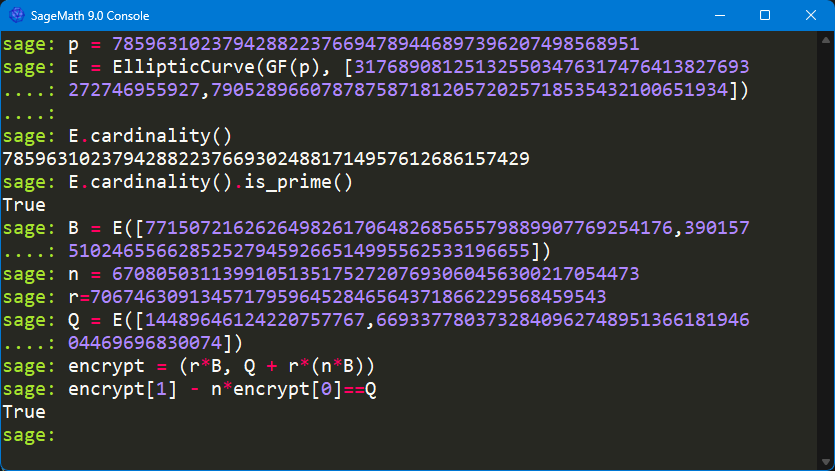
\includegraphics[width=0.8\textwidth]{C:/Users/dimit/Desktop/TeX/EC/drm}
\end{figure}

$ $\newline
Αν η \tl{Alice} ήξερε η ίδια το $n$ θα μπορούσε να υπολογίσει το $Q$ μόνη της και έτσι να μοιραστεί την μουσική με τον \tl{Bob}. Αυτό το κρυπτοσύστημα έσπασε, όχι γιατί δεν ήταν ασφαλές από μαθηματικής άποψης, αλλά γιατί είχε φτωχή υλοποίηση καθώς η ιδέα του ήταν να αποθηκεύει στον υπολογιστή του χρήστη το ιδιωτικό κλειδί. Περισσότερα για το συγκεκριμένο κενό ασφαλείας μπορεί να διαβάσει κανείς στο \tl{cryptome.org/ms-drm.htm}.
\pagebreak

\section{Ψηφιακές Υπογραφές}

\vspace*{0.3cm}
\noindent Οι ψηφιακές υπογραφές χρησιμοποιούν τα ίδια κρυπτοσυστήματα για την κρυπτογράφηση μηνυμάτων αλλά με διαφορετικό σκοπό. Δεν είναι το κίνητρο να περαστεί ασφαλώς το μήνυμα στον παραλήπτη, αλλά όπως το λέει η λέξη υπογραφή, είναι για να διασφαλιστούν τα ακόλουθα τρία πράγματα. Άρχικά είναι για την αυθεντικότητα των μηνυμάτων, να υπάρχει εξασφάλιση ότι βρίσκεται πράγματι το ίδιο άτομο που αναγράφεται πίσω από τα μηνύματα. Ο δεύτερος λόγος είναι μια απόδειξη ότι το αρχικό μήνυμα δεν έχει αλλοιωθεί και τελευταίος λόγος είναι ότι αυτός που υπέγραψε το μήνυμα δεν μπορεί στο μέλλον να το αρνηθεί.

$ $\newline
Το πρωτόκολλο λειτουργεί ως εξής, έχοντας συμφωνήσει σε ένα ασύμμετρο αλγόριθμο κρυπτογράφησης ο \tl{Bob} θέλει η \tl{Alice} να του υπογράψει ένα μήνυμα $m$. Στέλνει το $m$ στην \tl{Alice} και εκείνη μπλέκει το μήνυμα με το ιδιωτικό της κλειδί και του επιστρέφει το μήνυμα. Ο \tl{Bob} με την σειρά του μπλέκει το μήνυμα που έλαβε με το δημόσιο κλειδί της \tl{Alice} και του επιστρέφεται το αρχικό μήνυμα $m$. Φυσικά αυτό μπορεί να το κάνει οποιοσδήποτε κρυφακούει την συνομιλία. Δηλαδή, ακόμα και κάποιος που κρυφάκουσε μπορεί να επαληθέυσει ότι το μήνυμα το υπέγραψε η ίδια η \tl{Alice}.

\subsection{Αλγόριθμος Ψηφιακής Υπογραφής}

\vspace*{0.3cm}
Ο αλγόριθμος ψηφιακής υπογραφής γνωστός ως \tl{DSA} χρησιμοποιείται για υπογραφή και επαλήθευση υπογραφής. Ομοίως, η ασφάλεια του βασίζεται στην δυσκολία επίλυσης του προβλήματος διακριτού λογαρίθμου. Σαν αλγόριθμος, είναι μια παραλλαγή του κρυπτοσυστήματος \tl{El Gamal}. Λειτουργεί ως εξής:

\begin{itemize}
	\item Η χρήση του \tl{DSA} για υπογραφή αρχικά υπολογίζει το \tl{hash} του μηνύματος και παράγει έναν τυχαίο ακέραιο $k$. Με αυτά τα δύο υπολογίζει την υπογραφή $\{r,s\}$. Τα $r,s$ είναι ακέραιοι και το $r$ εξαρτάται μόνο από το $k$, ενώ το $s$ υπολογίζεται από το \tl{hash} του μηνύματος, το ιδιωτικό κλειδί του ασύμμετρου αλγορίθμου που χρησιμοποιούμε και τον τυχαίο αριθμό $k$. Εφόσον έχουμε τυχαιότητα με το $k$ αυτή η διαδικασία υπογραφής θεωρείται μη-ντετερμινιστική.
	\item Για την επαλήθευση της υπογραφής γίνονται υπολογισμοί, δεχόμενοι σαν είσοδο το \tl{hash} του μηνύματος, το δημόσιο κλειδί του ασύμμετρου αλγορίθμου καθώς και της ίδιας της υπογραφής $\{r,s\}$.
\end{itemize}

$ $\newline
Ο τυχαίος αριθμός $k$ (που παράγεται όταν δημιουργείται η υπογραφή) αφήνει ένα κενό ασφάλειας. Αν δύο διαφορετικά μηνύματα υπογραφούν με το ίδιο ιδιωτικό κλειδί και το ίδιο $k$ τότε ένας μπορεί να επιτεθεί στο πρωτόκολλο και να βρει το ιδιωτικό κλειδί του υπογραφέα. (Δες \tl{github.com/tintinweb/ecdsa-private-key-recovery}).

$ $\newline
Υπάρχει και ο περισσότερο ασφαλής ντετερμινιστικός \tl{DSA}, που δεν υπολογίζει το $k$ τυχαία αλλά σαν \tl{hash message authentication code (HMAC)} που εξαρτάται από το ιδιωτικό κλειδί, το \tl{hash} του μηνύματος που αποστέλλεται και άλλες παραμέτρους. Όπως θα δούμε, χρησιμοποιούνται οι ελλειπτικές καμπύλες με τέτοιο αλγόριθμο, βασιζόμενοι στην δυσκολία του \tl{ECDLP} καθώς και το μικρότερο μέγεθος σε μνήμη που έχουν τα κλειδιά και οι υπογραφές, ενώ ταυτόχρονα παρέχεται το ίδιο επίπεδο ασφάλειας και καλύτερη επίδοση. 

$ $\newline
Επιπλέον, το δημόσιο κλειδί $(x,y)$ της ελλειπτικής μπορεί πάντα να συμπυκνωθεί στο $x$. Αν για παράδειγμα έχουμε την καμπύλη \tl{secp256k1} που έχει ιδιωτικά κλειδιά με $256$-\tl{bit} ακεραίους (32 \tl{bytes}) τότε γνωρίζοντας το $x$, το $x^3+ax+b := m$ είναι γνωστό και έχουμε να υπολογίσουμε το τετραγωνικό υπόλοιπο:
$$y^2 = m \ \mod p$$ οπότε απλά κρατάμε ένα επιπλέον \tl{bit} για το πρόσημο μέσα στο τετράγωνο. Έτσι, έχουμε δημόσιο κλειδί με $257$-\tl{bit}. 

\subsection{Πρωτόκολλο ECDSA}

\vspace*{0.3cm}
\noindent Ο αλγόριθμος ψηφιακής υπογραφής ελλειπτικών καμπυλών \tl{(ECDSA)} είναι μια παραλλαγή του κλασικού \tl{DSA} και ομοίως στηρίζεται στο κρυπτοσύστημα \tl{El Gamal}. Για τον αλγόριθμο έχουμε ως είσοδο $(E,n,G,dG)$, όπου $E$ είναι μια ελλειπτική καμπύλη πάνω από κάποιο πεπερασμένο σώμα $\mathbb{F}_q$, $n$ είναι η τάξη της ομάδας που παράγει το $G\in E$ και είναι πρώτος αριθμός και $d \in \{2,\ldots, n-1\}$ το ιδιωτικό κλειδί το οποίο με την σειρά του δίνει το δημόσιο κλειδί $d G$.

\vspace*{0.3cm}
\begin{itemize}
	\item \textbf{Υπογραφή:}
	\begin{enumerate}
		\item Υπολογίζουμε το \tl{hash} του μηνύματος $m$, με κάποιον \tl{hash} αλγόριθμο όπως ο \tl{SHA-256}, παίρνουμε $h=hash(m)$.
		\item Παράγουμε τυχαία έναν ακέραιο αριθμό $k < n$, ή στην ντετερμινιστική περίπτωση παίρνουμε το \tl{HMAC} των $h,d$.
		\item Υπολογίζουμε το σημείο στην καμπύλη $R = kG$ και παίρνουμε την $x$ συντεταγμένη του ως $r = R.x$
		\item Υπολογίζουμε το $s = k^{-1} (h+rd) \ \mod n$, όπου $k^{-1}$ είναι το αντίστροφο του $k$ στο σώμα $\mathbb{Z}/n\mathbb{Z}$, δηλαδή $k k^{-1} = 1 \mod n$.
		\item Επιστρέφουμε την υπογραφή $\{r,s\}$.
	\end{enumerate}

	\vspace*{0.3cm}

	\item \textbf{Επαλήθευση Υπογραφής:}
	
	$ $\newline
	Παίρνουμε σαν είσοδο το μήνυμα $m$ που στάλθηκε για υπογραφή, την υπογραφή $\{r,s\}$ και το δημόσιο κλειδί $dG$ του υπογραφέα που αντιστοιχεί στο ιδιωτικό κλειδί $d$. Κατόπιν, εκτελούμε τα ακόλουθα:
	\begin{enumerate}
		\item Υπολογίζουμε το \tl{hash} του μηνύματος $m$, με τον ίδιο αλγόριθμο όπως πριν και έχουμε $h=hash(m)$.
		\item Υπολογίζουμε το $s^{-1} \in \mathbb{Z}/n \mathbb{Z}$.
		\item Υπολογίζουμε το σημείο στην ελλειπτική καμπύλη $R^{\prime} = (h s^{-1})\cdot G + (r s^{-1})\cdot dG = s^{-1}(h+rd) \cdot G$.
		\item Παίρνουμε ως $r^{\prime}$ την $x$-συντεταγμένη $r^{\prime} = R^{\prime}.x$.
		\item Επαληθεύουμε αν $r=r^{\prime}$.
	\end{enumerate}
\end{itemize}

$ $\newline
Ουσιαστικά, υπογράφοντας κωδικοποιείται ένα στοιχείο $R$ της ελλειπτικής καμπύλης (που αναπαρίσταται μόνο με την $x$-συντεταγμένη) ως $r$ και με πράξεις στην ελλειπτική καμπύλη χρησιμοποιώντας τα $d,h$ παίρνουμε το $s$. Το $s$ είναι το αποδεικτικό στοιχείο ότι αυτός που υπογράφει το μήνυμα γνωρίζει το ιδιωτικό κλειδί $d$. Έχοντας μόνο την υπογραφή $\{r,s\}$ είναι υπολογιστικά δύσκολο να βρεθεί το $d$, λόγω της δυσκολίας επίλυσης του \tl{ECDLP}.

$ $\newline
Για την επαλήθευση, αποδικωποιείται το $s$ πίσω στο αρχικό σημείο $R$ της ελλειπτικής καμπύλης χρησιμοποιώντας το δημόσιο κλειδί $dG$ και το \tl{hash} $h$. Στην συνέχεια, γίνεται η σύγκριση της $x$-συντεταγμένης με το $r$ της υπογραφής.

$ $\newline
Για του λόγου το αληθές, κάνουμε τις πράξεις για την ορθότητα της διαδικασίας. Έχουμε:
$$R^{\prime} = (h s^{-1})\cdot G + (r\cdot s^{-1})\cdot dG = s^{-1}(h+rd)\cdot G$$
και το $s$ κατά την διαδικασία της υπογραφής το έχουμε υπολογίσει ως:
$$s = k^{-1}(h+rd) \ \mod n$$ άρα
$$s^{-1} = (k^{-1}(h+rd))^{-1} = k(h+rd)^{-1} \ \mod n$$ και μπορούμε να κάνουμε την αντικατάσταση $s^{-1} \leftrightarrow k(h+rd)^{-1}$ στο $R^{\prime}$, τα αντίστροφα είναι απλά ακέραιοι $\mod n$ και εφόσον τα $s^{-1}, k(h+rd)^{-1}$ είναι ισοδύναμα $\mod n$ τότε θα δίνουν και το ίδιο σημείο στην καμπύλη ως συντελεστές του $G$, αφού η ομάδα στην οποία δουλεύουμε είναι η $\{\mathcal{O},G,2G,\ldots,(n-1)G\}$ που παράγεται από το $G$ με τάξη $n$. Άρα πράγματι μπορούμε να κάνουμε την αντικατάσταση:

$$R^{\prime} = s^{-1}(h+rd) \cdot G = k(h+rd)^{-1}(h+rd) \cdot G = kG = R$$ Συνεπώς, ο υπογραφέας είναι πράγματι αυτός που υποστηρίζει αν ισχύει ότι $r=r^{\prime}$ που σημαίνει ότι επαληθεύεται η σχέση $R=R^{\prime}$ και δεν έχει συμβεί κάποιο σφάλμα.

\vspace*{0.3cm}
\subsection{Ανάκτηση Δημόσιου Κλειδιού}

\vspace*{0.3cm}
\noindent Είναι αρκετά σημαντικό ότι με το πρωτόκολλο \tl{ECDSA} μπορεί το δημόσιο κλειδί να ανακτηθεί από το μήνυμα $m$ μαζί με την υπογραφή $\{r,s\}$. Αυτό επιτρέπει σε διάφορα συστήματα να μην μεταφέρουν το δημόσιο κλειδί, μειώνοντας έτσι το μέγεθος της πληροφορίας που ανταλλάσεται. Αυτό είναι ιδιαίτερα χρήσιμο εκεί που οι πόροι μοιράζονται με αυστηρό τρόπο και δεν θα θέλαμε να κρατάμε επιπλέον πληροφορία. Ένα παράδειγμα που συμβαίνει αυτό είναι στα \tl{blockchain} συστήματα. Εκεί τα δημόσια κλειδιά δεν αποθηκεύονται και ανακτούνται την στιγμή της επαλήθευσης των συναλλαγών. Ωστόσο, η διαδικασία της ανάκτησης με είσοδο $\{r,s\}$ επιτρέπει σε $0,1$ ή $2$ πιθανά δημόσια κλειδιά. Για να αποφεύγεται αυτό γίνεται μια επέκταση του \tl{ECDSA} που επιστρέφει σαν υπογραφή $\{r,s,v\}$ ένα επιπλέον \tl{bit} $v$ με το οποίο ανακτάται το δημόσιο κλειδί με σιγουριά. Με αυτόν τον τρόπο, το \tl{Ethereum} για παράδειγμα χρησιμοποιεί υπογραφές $\{r,s,v\}$ για τις υπογεγραμμένες συναλλαγές επιβαρύνοντας λιγότερο το δίκτυο και δεσμεύοντας λιγότερο αποθηκευτικό χώρο. 

$ $\newline
Έχοντας ως παραμέτρους τα $(E,G,n,k)$  με $E$ την ελλειπτική καμπύλη, $G$ το στοιχείο που διαλέγουμε σαν γεννήτορα τάξης $n$ και $k = |E|/n$, τότε για ένα μήνυμα $m$ με \tl{hash} $h$ και υπογραφή $\{r,s\}$ η ανάκτηση γίνεται ως εξής:

\vspace*{0.3cm}
\begin{enumerate}
	\item Για $j=0$ έως $k$:
	\begin{enumerate}
		\item Θέτουμε $x = r +jn$.
		\item Μετατροπή του ακεραίου $x$ σε \tl{octet string} $X$ όπως περιγράφεται στο \tl{SEC1} \cite{sec1}. %http://www.secg.org/sec1-v2.pdf
		\item Μετατροπή του \tl{octet string} $02_{16}||X$ σε σημείο $R$ της ελλειπτικής καμπύλης, όμοια όπως στο \cite{sec1}. Αν αποτύχει αυτό γύρνα στο βήμα $(1)$.
		\item Αν $nR\neq \mathcal{O}$ τότε γύρνα στο βήμα $(1)$.
		\item Πιθανό δημόσιο κλειδί:
		$$Q = r^{-1}(sR - hG)$$
		δοκιμή της επαλήθευσης αν μας επιστρέφει το μήνυμα $m$, αν ναι τέλος του αλγορίθμου και εκτυπώνεται το $Q$. Αν όχι, δοκιμάζουμε το ίδιο με το $-R$ αντί για το $R$.
	\end{enumerate}
	\item Αν τελειώσει η επανάληψη Για χωρίς να τελειώσει ο αλγόριθμος, εκτύπωσε ότι δεν υπάρχει δημόσιο κλειδί.
\end{enumerate}

\subsection{Κώδικας}

\vspace*{0.3cm}
\noindent Θα βασιστούμε στην βιβλιοθήκη \tl{ecdsa} που βρίσκεται στην βιβλιοθήκη \tl{pycoin} της γλώσσας προγραμματισμού \tl{Python}. Θα χρησιμοποιήσουμε τον αλγόριθμο \tl{hashing SHA3-256} και έναν γεννήτορα της ελλειπτικής καμπύλης \tl{Secp256k1}. Οι παραπάνω πράξεις και ελέγχοι που γίνονται για την υπογραφή και επαλήθευση είναι ήδη υλοποιημένες στις βιβλιοθήκες και τις χρησιμοποιούμε ως \tl{generator.sign(), generator.verify()}. Άρα μπορούμε να δούμε παρακάτω ένα παράδειγμα που υπογράφουμε ένα μήνυμα, κάνουμε επαλήθευση της υπογραφής και τι γίνεται αν παραλλάξουμε το μήνυμα:

\vspace*{0.3cm}
\begin{lstlisting}[language=Python]
from pycoin.ecdsa.secp256k1 import secp256k1_generator
import hashlib, secrets

def sha3_256Hash(msg):
	hashBytes = hashlib.sha3_256(msg.encode("utf8")).digest()
	return int.from_bytes(hashBytes, byteorder="big")

def signECDSAsecp256k1(msg, privKey):
	msgHash = sha3_256Hash(msg)
	signature = secp256k1_generator.sign(privKey, msgHash)
	return signature

def verifyECDSAsecp256k1(msg, signature, pubKey):
	msgHash = sha3_256Hash(msg)
	valid = secp256k1_generator.verify(pubKey, msgHash, \
	signature)
	return valid


# ECDSA sign message (using the curve secp256k1 + SHA3-256)
msg = "Message for ECDSA signing"
privKey = secrets.randbelow(secp256k1_generator.order())
signature = signECDSAsecp256k1(msg, privKey)
print("Message:", msg)
print("Private key:", hex(privKey))
print("Signature: r=" + hex(signature[0]) + ", s=" + \
hex(signature[1]))

# ECDSA verify signature (using the curve secp256k1 + SHA3-256)
pubKey = (secp256k1_generator * privKey)   	
valid = verifyECDSAsecp256k1(msg, signature, pubKey)
print("\nMessage:", msg)
print("Public key: (" + hex(pubKey[0]) + ", " + \ 
hex(pubKey[1]) + ")")
print("Signature valid?", valid)

# ECDSA verify tampered signature 
#(using the curve secp256k1 + SHA3-256)
msg = "Tampered message"
valid = verifyECDSAsecp256k1(msg, signature, pubKey)
print("\nMessage:", msg)
print("Signature (tampered msg) valid?", valid)
\end{lstlisting}

\begin{figure}[H]
	\centering
	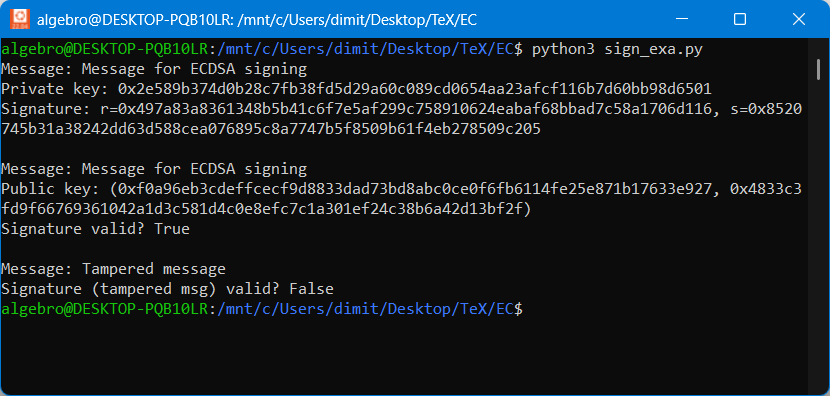
\includegraphics[width=1\textwidth]{C:/Users/dimit/Desktop/TeX/EC/sign_pic}
\end{figure}

$ $\newline
Στα παραπάνω, αν ορίσουμε την ακόλουθη συνάρτηση:

\vspace*{0.3cm}
\begin{lstlisting}[language = Python]
def recoverPubKeyFromSignature(msg, signature):
    msgHash = sha3_256Hash(msg)
    recoveredPubKeys = 
	secp256k1_generator.possible_public_pairs_for_signature(
	msgHash, signature)
    return recoveredPubKeys
\end{lstlisting}

$ $\newline
και τρέξουμε το ακόλουθο κομμάτι:

\vspace*{0.3cm}
\begin{lstlisting}[language=Python]
msg = "Message for ECDSA signing"
privKey = secrets.randbelow(secp256k1_generator.order())
signature = signECDSAsecp256k1(msg, privKey)

recoveredPubKeys = recoverPubKeyFromSignature(msg, signature)
print("\nMessage:", msg)
print("Signature: r=" + hex(signature[0]) + ", s=" + \
hex(signature[1]))
for pk in recoveredPubKeys:
    print("Recovered public key from signature: (" +
          hex(pk[0]) + ", " + hex(pk[1]) + ")")
\end{lstlisting}

$ $\newline
παίρνουμε ένα αποτέλεσμα σαν το ακόλουθο:

\vspace*{0.3cm}
\begin{figure}[H]
	\centering
	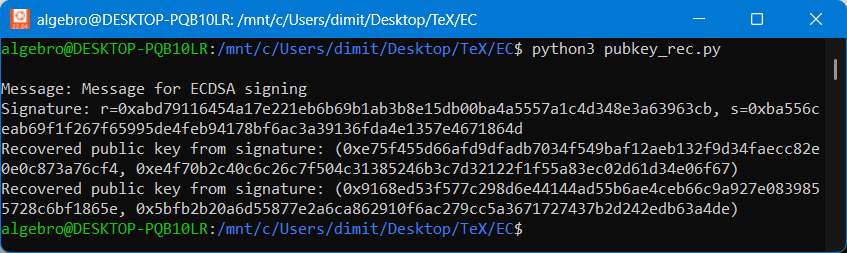
\includegraphics[width=1\textwidth]{C:/Users/dimit/Desktop/TeX/EC/pubkey_rec_pic}
\end{figure}

$ $\newline
Όπως είναι αναμενόμενο, θα είναι δύο τα δημόσια κλειδιά που ταιριάζουν με την υπογραφή και το μήνυμα ταυτόχρονα. Το ένα θα είναι το σωστό που θα ταιριάζει και με το ιδιωτικό κλειδί, ενώ το άλλο απλά ταιριάζει στα μαθηματικά της ανάκτησης του δημοσίου κλειδιού. Δηλαδή, όπως παραπάνω που δοκιμάζουμε το $R$ ή το $-R$, ουσιαστικά αν $R= (x,y)$ τότε $-R  =(x,-y)$ πάνω στην ελλειπτική καμπύλη, δηλαδή δεν ξέρουμε το πρόσημο του $y$ το οποίο κρατάμε ως $v$ στην γενικευμένη υπογραφή $\{r,s,v\}$. Ας δούμε ένα παράδειγμα με \tl{extended ecdsa}. Θα χρησιμοποιήσουμε την βιβλιοθήκη \tl{eth keys} που είναι μέρος του \tl{Ethereum} και χρησιμοποιεί κρυπτογραφία ελλειπτικών καμπυλών με βάση την καμπύλη \tl{secp256k1} για ιδιωτικά και δημόσια κλειδιά, καθώς και γενικευμένες \tl{ECDSA} υπογραφές $\{r,s,v\}$.

\vspace*{0.3cm}
\selectlanguage{english}
\begin{lstlisting}
import eth_keys, os

# Generate the private + public key pair
# (using the secp256k1 curve)
signerPrivKey = eth_keys.keys.PrivateKey(os.urandom(32))
signerPubKey = signerPrivKey.public_key
print('Private key (64 hex digits):', signerPrivKey)
print('Public key (uncompressed, 128 hex digits):', signerPubKey)

# ECDSA sign message (using the curve secp256k1 + Keccak-256)
msg = b'Message for signing'
signature = signerPrivKey.sign_msg(msg)
print('Message:', msg)
print('Signature: [r = {0}, s = {1}, v = {2}]'.format(
    hex(signature.r), hex(signature.s), hex(signature.v)))

# ECDSA public key recovery from signature + verify signature
# (using the curve secp256k1 + Keccak-256 hash)
msg = b'Message for signing'
recoveredPubKey = signature.recover_public_key_from_msg(msg)
print('Recovered public key (128 hex digits):', recoveredPubKey)
print('Public key correct?', recoveredPubKey == signerPubKey)
valid = signerPubKey.verify_msg(msg, signature)
print("Signature valid?", valid)
\end{lstlisting}

\begin{figure}[H]
	\centering
	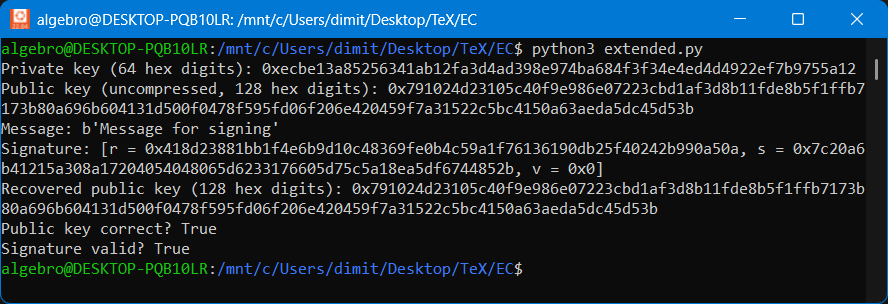
\includegraphics[width=1\textwidth]{C:/Users/dimit/Desktop/TeX/EC/extended_pic}
\end{figure}

$ $\newline
Εδώ φυσικά θα παίρνουμε πίσω το δημόσιο κλειδί με σιγουριά και η επαλήθευση της υπογραφής θα είναι επιτυχής. Εκτός αν αλλοιωθεί με κάποιο τρόπο το μήνυμα, ή το δημόσιο κλειδί, ή αλλιώς η υπογραφή.

\pagebreak
\section{\tl{Vulnerabilities}}

\vspace*{0.3cm}
\noindent Παραπάνω έχουμε δει ότι χρησιμοποιούνται συγκεκριμένες καμπύλες όπως η \tl{NIST P}-256 και η \tl{secp256k1} που έχουν συγκεκριμένες παραμέτρους. Θα μπορούσαμε να ορίζουμε οποιαδήποτε ελλειπτική καμπύλη και να κάνουμε κρυπτογραφία? Η αλήθεια είναι πως αυτό δεν θα ήταν ασφαλές. Όπως θα αναφερθούν παρακάτω, υπάρχουν διάφορα κρυπτογραφικά πρότυπα που πρέπει να ικανοποιεί μια καμπύλη για να θεωρείται ασφαλής. Ας δούμε μερικά σενάρια ελλειπτικών καμπυλών που οι παραμέτροι τους τις καθιστούν μη ασφαλείς για κρυπτογραφία.

\vspace*{0.3cm}
\subsection{Επίθεση \tl{Pohlig-Hellman}}

\vspace*{0.3cm}
Ας υποθέσουμε ότι έχουμε μια ελλειπτική καμπύλη $E(\mathbb{F}_p)$ και γεννήτορα $P$ με τάξη $n=p_1^{r_1} p_2^{r_2} \cdots p_s^{r_s}$, όπου οι $p_i$ είναι πρώτοι αριθμοί και σχετικά μικροί σε μέγεθος. Η επίθεση \tl{Pohlig - Hellman} ουσιαστικά μεταφέρει το πρόβλημα \tl{ECDLP} από το $E(\mathbb{F}_p)$ που είναι δύσκολο στις υποομάδες της $\langle G \rangle$ με τάξη πρώτο αριθμό. Σε κάθε τέτοια υποομάδα είναι αρκετά πιο εύκολο το πρόβλημα και αφού λυθεί, στο τέλος λύνεται το αρχικό πρόβλημα χρησιμοποιώντας το κινέζικο θεώρημα υπολοίπων.

$ $\newline
Υποθέτουμε ότι η τάξη του $P$ έχει την προηγούμενη παραγοντοποίηση και έχοντας το σημείο $Q = kP$ θέλουμε να υπολογίσουμε το $k$. Αρκεί να βρούμε αριθμούς $k_i$ τέτοιους ώστε:
$$k_i =  k \mod p_i^{r_i}$$ και αυτό θα γίνει με το να τους γράψουμε στην μορφή:
$$k_i = z_0 + z_1 p_i + \cdots + z_{r_i -1} p_i^{r_i - 1}$$ και να υπολογίσουμε τα $z_j$ που αντιστιχούν στο κάθε $k_i$. Θέτουμε:

$$P_0 = \frac{n}{p_i}P \ \text{ και } \ Q_0 = \frac{n}{p_i} Q$$ Το $P_0$ έχει τάξη $p_i$ αφού $p_i P_0 = n P = \mathcal{O}$ και το $p_i$ είναι πρώτος, άρα δεν έχει μικρότερο διαιρέτη σαν πιθανή τάξη.

$$Q_0 = \frac{n}{p_i} kP = k\left( \frac{n}{p_i} P \right) = k P_0$$ και καθώς η τάξη του $P_0$ είναι $p_i$ και $z_0$ ο πρώτος συντελεστής του $k_i$ στην $p_i$-αδική αναπαράσταση, έχουμε ότι
$$k P_0 = k_i P_0 =  z_0 P_0 + z_1 p_i P_0 + \cdots + z_{r_i-1}p_i^{r_i-1}P_0 = z_0 P_0 = Q_0$$ όπου η προηγούμενη αντικατάσταση $k = k_i = z_0$ ισχύει αφού σε όλα γίνονται $\mod p_i$ στην κυκλική ομάδα $\langle P_0 \rangle$ τάξης $p_i$. Οπότε, σε αυτήν την υποομάδα τάξης $p_i$ έχει να λυθεί το αρκετά πιο εύκολο \tl{ECDLP} $P_0 = z_0 Q_0$. Γενικεύοντας αυτό το επιχείρημα παίρνουμε όλα τα $z_j$ που εμφανίζονται στην $p_i$-αδική αναπράσταση του $k_i$ ως εξής:

$$Q_j = \frac{n}{p_i^{j+1}}\left(Q - z_0 P - z_1 p_i P - z_2 p_i^2 P - \cdots - z_{j-1} p_i^{j-1} P\right)$$ Συνεπώς, κάνοντας την ίδια διαδικασία για τα διαφορετικά $p_i$ παίρνουμε το σύστημα εξισώσεων:

\begin{align*}
	k &= k_1 \ \mod p_1^{r_1} \\
	k &= k_2 \ \mod p_2^{r_2} \\
	k &= k_3 \ \mod p_3^{r_3} \\
	& \quad  \quad \quad \vdots  \\
	k &= k_s \ \mod p_s^{r_s} 
\end{align*}

$ $\newline
Το οποίο μπορούμε να λύσουμε με το κινέζικο θεώρημα υπολοίπων, αφού όλα τα $p_i^{r_i}$ είναι σχετικά πρώτα ανά δύο. Έτσι, υπολογίζουμε το $k$ και λύνουμε σε αυτή τη περίπτωση το αρχικό \tl{ECDLP}. Ας δούμε αυτό το παράδειγμα υπολογιστικά. Ο παρακάτω κώδικας για το \tl{SageMath} είναι από τον \tl{Peter Novotney} \cite{novotney}.

\vspace*{0.3cm}
\begin{sageblock}
	def PohligHellman(P,Q):
....:     zList = list()
....:     conjList = list()
....:     rootList = list()
....:     n = P.order()
....:     factorList = n.factor()
....:     for facTuple in factorList:
....:         P0 = (ZZ(n/facTuple[0]))*P
....:         conjList.append(0)
....:         rootList.append(facTuple[0]^facTuple[1])
....:         for i in range(facTuple[1]):
....:             Qpart = Q
....:             for j in range(1,i+1):
....:                 Qpart = Qpart -(zList[j-1]*(facTuple[0]^(j-1))*P)
....:             Qi = (ZZ(n/(facTuple[0]^(i+1))))*Qpart
....:             zList.insert(i,discrete_log(Qi,P0,operation='+'))
....:             conjList[-1]=conjList[-1]+zList[i]*(facTuple[0]^i)
....:     return crt(conjList,rootList)
\end{sageblock}

$ $\newline
Και ας δούμε ένα μικρό και ένα λίγο πιο μεγάλο παράδειγμα:

\vspace*{0.3cm}
\begin{figure}[H]
	\centering
	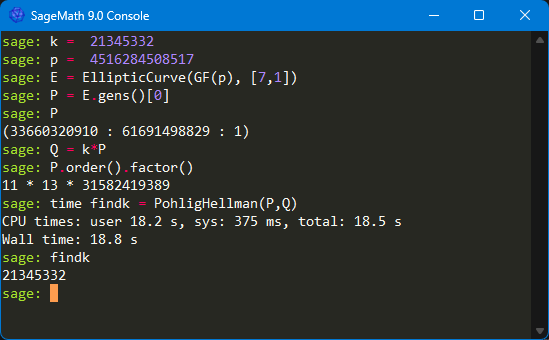
\includegraphics[width=0.7\textwidth]{C:/Users/dimit/Desktop/TeX/EC/PH_baby}
	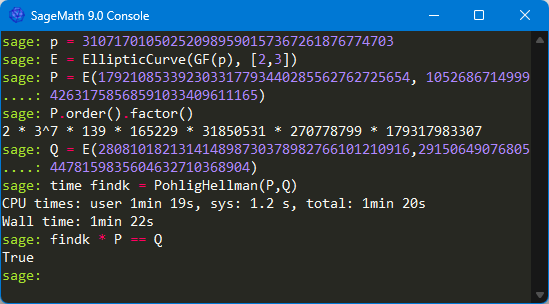
\includegraphics[width=0.7\textwidth]{C:/Users/dimit/Desktop/TeX/EC/PH_big}
\end{figure}

$ $\newline
Όπως βλέπουμε, σε μια τέτοια κακή επιλογή παραμέτρων το \tl{ECDLP} είναι όσο δύσκολο είναι το \tl{DLP} στην κυκλική ομάδα με τάξη τον μεγαλύτερο διακεκριμένο πρώτο αριθμό που εμφανίζεται στην παραγοντοποίηση της τάξης του γεννήτορα $P$.

$ $\newline
Ας κάνουμε μια παραλλαγή και ας υποθέσουμε ότι στην παραγοντοποίηση $n = p_1^{r_1} p_2^{r_2} \cdots p_s^{r_s}$ ο πρώτος $p_s$ είναι αρκετά μεγάλος για να λύνεται γρήγορα το πρόβλημα του διακριτού λογαρίθμου στην αντίστοιχη κυκλική ομάδα, ενώ οι υπόλοιποι διακεκριμένοι πρώτοι είναι αρκετοί και με μέγεθος που λύνεται το αντίστοιχο πρόβλημα σχετικά γρήγορα στον καθένα. Αν είχαμε την πληροφορία ότι το ιδιωτικό κλειδί είναι σχετικά μικρό σε μέγεθος, γιατί θα μπορούσε να είναι φτωχή υλοποίηση ή να απευθύνεται σε μικρές συσκευές, τότε θα υπήρχε μεγάλη πιθανότητα στην παραπάνω διαδικασία να μπορούσαμε να παραλείψουμε τον πρώτο $p_s$. Δηλαδή, να κρατούσαμε τις εξισώσεις:
\begin{align*}
	k &= k_1 \ \mod p_1 \\
	k &= k_2 \ \mod p_2 \\
	& \quad \quad \quad \vdots \\
	k &= k_{s-1} \ \mod p_{s-1}
\end{align*}

$ $\newline
και με το κινέζικο θεώρημα να προέκυπτε η λύση $k=a \ \mod M$. Εδώ θα μπορούσε το $M$ να είναι αρκετά μεγάλο που να μας διασφάλιζε ότι $k=a$. Δηλαδή, αν θεωρητικά είχαμε συμπεριλάβει την εξίσωση $k=k_s \ \mod p_s$ στο κινέζικο θεώρημα υπολοίπων, απλά θα παίρναμε ότι $k = a \ \mod M^{\prime}$ για κάποιο $M^{\prime}>M$. Σε αυτήν την παραλλαγή, δηλαδή με την έξτρα πληροφορία ότι το ιδιωτικό κλειδί είναι σχετικά μικρό σε μέγεθος, μπορούμε να το βρούμε χωρίς να λύσουμε το \tl{ECDLP} για κάθε υποομάδα με τάξη πρώτο, αλλά ακριβώς για όσες αρκεί. Ενδεχομένως, θα αποφεύγαμε τους πολύ μεγάλους πρώτους αριθμούς στην παραγοντοποίηση της τάξης του γεννήτορα. 

\vspace*{0.3cm}
\subsection{Ανώμαλες Καμπύλες}

\vspace*{0.3cm}
\noindent Όπως είδαμε στα προηγούμενα κεφάλαια, είναι αρκετά βολικό η τάξη του γεννήτορα $P$ να είναι πρώτος αριθμός. Όπως φαίνεται από την επίθεση \tl{Pohlig-Hellman}, για περισσότερη ασφάλεια πρέπει αυτός ο πρώτος να είναι σχετικά μεγάλος. Τι γίνεται αν δοκιμάσει κανείς να κάνει κρυπτογραφία με μια ελλειπτική καμπύλη $E(\mathbb{F}_p)$ που είναι κυκλική και έχει γεννήτορα $P$ με τάξη το ίδιο το $p$ του σώματος? Μια τέτοια καμπύλη ονομάζεται στην βιβλιογραφία ανώμαλη ελλειπτική καμπύλη.

$ $\newline
Η ιδέα εδώ είναι ότι το \tl{ECDLP} θα μεταφερθεί ως μια εξίσωση στο σώμα $\mathbb{F}_p$ που λύνεται τετριμμένα. Αρκεί δηλαδή να βρεθεί ένας ισομορφισμός ομάδων:
$$\phi : E(\mathbb{F}_p) \longrightarrow \mathbb{F}_p$$
Ορίζουμε ένα ευθύ άθροισμα:

$$E(\mathbb{F}_p) \oplus \mathbb{F}_p$$ με πράξη πρόσθεσης:
$$(Q_1,a) \oplus (Q_2,b) = (Q_1+Q_2, a+b+\lambda (Q_1,Q_2))$$ όπου $\lambda(Q_1,Q_2)$ είναι η κλίση της ευθείας που περνάει από τα $Q_1, Q_2$ ή της εφαπτομένης αν $Q_1 = Q_2$. Αν ένα από τα δύο είναι το $\mathcal{O}$, τότε παίρνουμε την τιμή $0$. Έχοντας ότι $p Q = \mathcal{O}$ για κάθε $Q \in E$ τότε:

$$p[Q,0] = [Q,0] \oplus [Q,0] \oplus \cdots \oplus [Q,0] = $$
$$[\mathcal{O}, \lambda(Q,Q) + \lambda(2Q,Q) + \cdots + \lambda((p-1)Q,Q)] :=[\mathcal{O},a]$$
$$\phi(Q) := a$$ και από την βιβλιογραφία \cite{semaev} αυτή η $\phi$ είναι καλά ορισμένη και είναι ο ζητούμενος ισομορφισμός ομάδων. Έτσι, έχουμε:



$$k P = Q \implies $$
$$k \phi(P) = \phi(Q) \implies $$
$$k = \phi(Q) \phi(P)^{-1} \in \mathbb{F}_p$$ το οποίο λύνεται τετριμμένα.



\vspace*{0.3cm}
\subsection{\tl{Singular} Καμπύλες}

\vspace*{0.3cm}
\noindent Στον ορισμό μιας ελλειπτικής καμπύλης $y^2 = x^3 + c_1 x +c_2$ δώσαμε την σχέση $16(4c_1^3 +27c_2^2)\neq 0$, δηλαδή της διακρίνουσας ενός πολυωνύμου τρίτου βαθμού να μην είναι $0$. Αυτό είναι ισοδύναμο με το πολυώνυμο $x^3 +c_1 x+c_2$ να έχει μόνο απλές ρίζες στο σώμα που το βλέπουμε και σε κάθε επέκτασή του. Τι θα γινόταν αν κάποιος επιχειρούσε να κάνει κρυπτογραφία με μια τέτοια καμπύλη που μοιάζει με ελλειπτική και το πολυώνυμο $x^3 + c_1x+c_2$ έχει πολλαπλές ρίζες; Τέτοιες καμπύλες τις συναντά κανείς στην αλγεβρική γεωμετρία και λέγονται \tl{singular}. Τα αντίστοιχα σημεία με πολλαπλές ρίζες λέγονται \tl{singular points}. Αυτές οι καμπύλες μπορούν να προκύψουν εντελώς φυσιολογικά κοιτώντας ελλειπτικές καμπύλες πάνω από το $\mathbb{Q}$ με $\Delta \neq 0$ και κάνοντας αναγωγή $\mod p$ με $\Delta = 0 \mod p$ προκύπτει πλέον μια καμπύλη που δεν είναι ελλειπτική πάνω από το $\mathbb{F}_p$.

$ $\newline
Ουσιαστικά, σε ένα \tl{singular} σημείο η καμπύλη θα διασταυρώνεται μεταξύ της και έτσι δεν θα μπορεί να οριστεί η εφαπτομένη για να χρησιμοποιήσουμε τον κανόνα πρόσθεσης σημείων. Ωστόσο, αν πετάξουμε τα \tl{singular} σημεία και κρατήσουμε όλα τα υπόλοιπα της ελλειπτικής μας μένει πάλι μια αβελιανή ομάδα που την συμβολίζουμε με $E_{ns}$. Έχουμε δύο περιπτώσεις:
$$y^2 = x^3+c_1 x+c_2 = f(x), \quad f(x) \in \mathbb{F}_p[x]$$
$$f(x) = (x-a)^3 \ \text{ ή } \ f(x) = (x-a)^2(x-b)$$

$ $\newline
Η πρώτη περίπτωση είναι τετριμμένη καθώς έχουμε το μόνο \tl{singular} σημείο $(a,0)$ και έτσι για την ομάδα $E_{ns}$ ισχύει ότι:
$$E_{ns} \simeq (\mathbb{F}_p,+)$$ η οποία είναι προσθετική, πράγμα που κάνει άμεση την επίλυση του διακριτού αλγορίθμου.

$ $\newline
Στην δεύτερη περίπτωση, η ομάδα $E_{ns}$ θα έχει τάξη $p-1$ ή $p+1$, δηλαδή θα είναι ισόμορφη με μια από τις πολλαπλασιαστικές $\mathbb{F}_p^{\times}$ ή $\mathbb{F}_{p^2}^{\times}$. Σε αυτήν την περίπτωση θα ορίζονται δύο ευθείες που προσπαθούν να πάρουν τον ρόλο της εφαπτομένης, οι οποίες είναι οι:

$$\varepsilon_1 : y = \sqrt{a-b}(x-a) \ \text{ και } \ \varepsilon_2 : y=-\sqrt{a-b}(x-a)$$ και με βάση αυτές ορίζεται ο ομομορφισμός ομάδων:

$$\phi : E_{ns} \longrightarrow \overline{\mathbb{F}_p} = \bigcup\limits_{i\geq 1} \mathbb{F}_{p^i}$$
$$(x,y) \longmapsto \frac{y+\sqrt{a-b}(x-a)}{y-\sqrt{a-b}(x-a)}$$ όπου $\overline{\mathbb{F}_p}$ είναι η αλγεβρική θήκη του $\mathbb{F}_p$ με πράξη τον πολλαπλασιασμό. Άρα αν θέλουμε να λύσουμε τον διακριτό λογάριθμο $P = kQ$ τότε θα έχουμε:
$$\phi(P)=\phi(Q)^k$$

$ $\newline
και το πρόβλημα ανάγεται στο να λυθεί ο διακριτός λογάριθμος στην πολλαπλασιαστική ομάδα $\mathbb{F}^{\times}_p$ ή στην $\mathbb{F}^{\times}_{p^2}$, ανάλογα σε ποιο από τα $\mathbb{F}_p, \mathbb{F}_{p^2}$ βρίσκονται τα $\phi(P),\phi(Q) \in \overline{\mathbb{F}_p}$. Αν το $a-b$ είναι τετράγωνο τότε το $\sqrt{a-b}$ θα βρίσκεται στο μικρότερο σώμα $\mathbb{F}_p$, διαφορετικά θα είναι στο $\mathbb{F}_{p^2}$. Εν κατακλείδι, εφόσον οι πολλαπλασιαστικές ομάδες πεπερασμένων σωμάτων είναι κυκλικές, η δυσκολία του διακριτού λογαρίθμου σε \tl{singular} καμπύλες ανάγεται στην δυσκολία που έχει ο διακριτός λογάριθμος σε μια κυκλική ομάδα τάξης $p-1$ ή αντίστοιχα $p+1$, το οποίο υπολογίζεται γρήγορα εφόσον το $p-1$ ή αντίστοιχα το $p+1$ δεν έχει σχετικά μεγάλου μεγέθους πρώτο παράγοντα.  
Περισσότερες λεπτομέρειες δίνουν στα βιβλία τους οι \tl{Silverman} \cite{silverman} και \tl{Washington} \cite{washington} στις σελίδες 55-58 και 59-64 αντίστοιχα.



%Elliptic Curves: Number Theory and Cryptography, second edition, Washington, pp 59-64
%The Arithmetic of Elliptic Curves, Silverman, pp 55-58

\subsection{Επίθεση \tl{MOV}}
%https://people.cs.nctu.edu.tw/~rjchen/ECC2009/19_MOVattack.pdf
%https://crypto.stanford.edu/pbc/notes/elliptic/movattack.html
%https://crypto.stackexchange.com/questions/1871/how-does-the-mov-attack-work

\vspace*{0.3cm}
\noindent Μια ιδιαίτερη επίθεση στο πρόβλημα \tl{ECDLP} είναι αυτή των \tl{A. Menezes, T. Okamoto} και \tl{S. Vanstone} \cite{mov}. Η ιδέα είναι να μεταφέρουμε το πρόβλημα διακριτού λογαρίθμου από το $E(\mathbb{F}_p)$ στο $\mathbb{F}_p^k$ για μικρό $k$ ώστε να λύνεται έυκολα. Για παράδειγμα, μια ελλειπτική καμπύλη πάνω από το $\mathbb{F}_p$ με $p$ να είναι της τάξης των 256 \tl{bit} προσφέρει ασφάλεια $128$ \tl{bit}, δηλαδή χρειάζονται $2^{128}$ βήματα στην επίθεση. Αλλά, αν το $k$ είναι δύο, τότε το πρόβλημα εμφυτεύεται στο $\mathbb{F}_p^2$ που παρέχει μόνο $60$ \tl{bit} ασφάλειας. Ουσιαστικά, η επίθεση βασίζεται σε μια συγκεκριμένη μη-εκφυλισμένη, εναλλάσουσα, πολλαπλασιαστικά διγραμμική μορφή με το όνομα ζευγάρωμα \tl{Weil}. Η διγραμμική μορφή αυτή έχει περίπλοκους ορισμούς στην βιβλιογραφία, αλλά στην ουσία παίρνει στοιχεία από τις ομάδες στρέψης $E[n]= \{P \in E: \ nP = \mathcal{O}\}$ και τα απεικονίζει σε ρίζες της μονάδας στην αλγεβρική θήκη του σώματος $K$ με χαρακτηριστική μεγαλύτερη του $0$, εφόσον $\text{μκδ}(n,char(K)) = 1$. Δηλαδή:

$$e: E[n]\times E[n] \longrightarrow \{x\in \overline{K}: x^n = 1\}$$ με τις ιδιότητες:

\begin{itemize}
	\item $e(rP,sQ) = \left(e(P,Q)\right)^{rs}$ για κάθε $P,Q \in E[n]$ και $r,s\in \mathbb{N}$.
	\item $e(P_1 + P_2, Q) = e(P_1,Q)\cdot e(P_2,Q)$
	\item $e(P, Q_1 + Q_2) = e(P,Q_1)\cdot e(P,Q_2)$
	\item $e(P,P) = 1$
	\item $e(P,Q) = e(Q,P)^{-1}$
	\item $e(P,Q) = 1$ για κάνε $Q$ αν και μόνο αν $P=\mathcal{O}$.
	\item $e(P,Q) = 1$ για κάθε $P$ αν και μόνο αν $Q = \mathcal{O}$.
\end{itemize}

$ $\newline
Θέλουμε να λύσουμε το \tl{ECDLP} με γεννήτορα $P$ με τάξη $n$ και σημείο $xP$. Υποθέτουμε ότι έχουμε ένα $Q \in E[n]$ που δεν ανήκει στην κυκλική ομάδα που ορίζει το $P$. Με άλλα λόγια, τα $P,Q$ είναι γραμμικά ανεξάρτητα με την έννοια ότι δεν υπάρχει φυσικός αριθμός $m$ με $Q=mP$. Τότε μπορούν να υπολογιστούν τα ακόλουθα:
$$e(P,Q) \text{ και } e(xP,Q) = e(P,Q)^x $$ και είναι και τα δύο $n$-οστές ρίζες της μονάδας. Εφόσον, τα $P,Q$ είναι γραμμικά ανεξάρτητα και η $e$ είναι μη-εκφυλισμένη τότε $e(P,Q) \neq 1$. Άρα πράγματι μεταφέρθηκε το πρόβλημα από \tl{ECDLP} σε \tl{DLP} στην πολλαπλασιαστική ομάδα του σώματος $K$. Για $K=\mathbb{F}_p$ έχουμε $\overline{\mathbb{F}_p} = \cup_{i\geq 1}\mathbb{F}_{p^i}$ και θέλουμε να περιοριστούμε όσο το δυνατόν γίνεται σε μικρότερο σώμα, το οποίο το πετυχάνουμε στο
$$\mathbb{F}_{p^{\ell}}, \quad \text{ όπου } \ell = \min\{ m \in \mathbb{N}: \ p^m = 1  \ \mod |E|\}$$ και εκεί γίνεται η επίθεση με μεθόδους όπως στην \tl{Pohlig-Hellman} που σπάει το πρόβλημα διακριτού λογαρίθμου σε μικρότερα προβλήματα και στο τέλος γίνεται σύνθεση της λύσης με το κινέζικο θεώρημα υπολοίπων. Επιπλέον, για μια τάξη ελλειπτικών καμπυλών με το όνομα υπεριδιάζουσες (\tl{supersingular}) ενώ το αρχικό πρόβλημα \tl{ECDLP} είναι αρκετά δύσκολο, με την παραπάνω διαδικασία γίνεται αρκετά εύκολο καθώς πετυχαίνεται η τιμή $\ell = 2$.

%https://crypto.stackexchange.com/questions/1871/how-does-the-mov-attack-work reference?
%https://crypto.stanford.edu/pbc/notes/elliptic/movattack.html reference?



\subsection{\tl{CurveΒall}}

\vspace*{0.3cm}
Τα προηγούμενα \tl{Vulnerabilities} αποτελούν πλέον εκπαιδευτικά παραδείγματα παρά κάτι που θα συναντήσει κανείς, εφόσον υπάρχουν τα στάνταρ που ελέγχονται για το ποιες ελλειπτικές καμπύλες χρησιμοποιούνται. Ωστόσο, υπήρξε ένα ιδιαίτερα εύκολο από μαθηματικής άποψης κενό ασφαλείας σε υλοποίηση της \tl{Microsoft} που βρέθηκε μόλις το \tl{2020}. Στο κενό δώθηκαν τα ονόματα \tl{CurveBall} και \tl{Chain of Fools}, το πρώτο κυρίως για την μαθηματική πράξη πάνω στην καμπύλη, ενώ το δεύτερο καθώς το κενό έχει να κάνει με πολλές ψηφιακές υπογραφές.
%https://blog.lessonslearned.org/chain-of-fools/
%https://github.com/IIICTECH/-CVE-2020-0601-ECC---EXPLOIT
%https://news.ycombinator.com/item?id=22048619
%https://www.youtube.com/watch?v=8RI60aRyhoE
%https://research.kudelskisecurity.com/2020/01/15/cve-2020-0601-the-chainoffools-attack-explained-with-poc/


%https://github.com/kudelskisecurity/chainoffools
$ $\newline
Αυτό που συνέβη ήταν ότι υπήρχε κενό στον έλεγχο και στον τρόπο που επαλήθευε τις \tl{ECC} υπογραφές το \tl{Windows CryptoAPI} στο αρχείο \tl{Crypt32.dll}. Ένας κακόβουλος χρήστης μπορούσε να εκμεταλλευτεί το κενό και να υπογράψει ένα δικό του κακόβουλο αρχείο και να φαίνεται σε όλους ότι η υπογραφή είναι από μια έμπιστη πηγή. Έτσι ο οποιοσδήποτε χρήστης μετά θα βασιζόταν στην πλέον έμπιστη υπογραφή και δεν θα μπορούσε να ξέρει ότι το λογισμικό που έχει λάβει είναι κακόβουλο. Το κενό που υπήρχε πραγματικά ήταν ότι τα \tl{Windows} έκαναν έλεγχο αν τους δίνεται η δεδομένη γνωστή καμπύλη και αν το δημόσιο κλειδί και άλλες παραμέτροι ήταν εντάξει, αλλά δεν γινόταν έλεγχος στο ποιος γεννήτορας της καμπύλης δίνεται. 

$ $\newline
Τα μαθηματικά είναι πιο απλά από όλα τα προηγούμενα παραδείγματα, παρόλο που αυτό είναι πραγματικό σενάριο. Ας υποθέσουμε ότι χρησιμοποείται η καμπύλη $P$-256 με τον γεννήτορα $G$ και ότι η \tl{Microsoft} έχει δημόσιο κλειδί $Q = xG$. Άν υποθέσουμε ότι ο $A$ ήθελε να επιτεθεί, θα μπορούσε να ορίσει την ίδια ακριβώς καμπύλη και τις παραμέτρους της, διασφαλίζοντας ότι περνάει τους ελέγχους έτσι, αλλά με διαφορετικό γεννήτορα. Ο $A$ δεν έχει καμία ελπίδα να ξέρει το ιδιωτικό κλειδί $x$ της \tl{Microsoft}, αλλά φτιάχνει το δικό του ιδιωτικό κλειδί $x^{\prime}$ και δίνει στο \tl{CryptoAPI} τον γεννήτορα:

$$G^{\prime} = (x^{\prime})^{-1} Q$$

$ $\newline
Έτσι, το \tl{CryptoAPI} βλέπει ότι
$$Q = x^{\prime} G^{\prime}$$ και άρα νομίζει ότι το ιδιωτικό κλειδί που αντιστοιχεί στο $Q$ είναι το $x^{\prime}$ που ξέρει ο $A$, ενώ είναι το $x$ της \tl{Microsoft}. Άρα πλέον ο $A$ θεωρείται έμπιστος ως η ίδια η \tl{Microsoft}. Μια περιγραφή των γεγονότων μπορεί να διαβάσει κανείς στο \tl{blog.lessonslearned.org/chain-of-fools/}.


$ $\newline
Εδώ είναι ακόμα πιο ξεκάθαρο, ότι όσο εκλεπτυσμένα και να είναι τα μαθηματικά πίσω από την κρυπτογραφία, το πρόβλημα μαθηματικής δυσκολίας είτε θα σπάει από εξωτερικούς παράγοντες, είτε θα μπορεί να παραβλέπεται τελείως και η κρυπτογραφία θα καταρρέει λόγω λανθασμένων φτωχών υλοποιήσεων.



\pagebreak
\section{Ασφαλείς Ελλειπτικές Καμπύλες}
%παράδειγμα υπογραφής google
%https://datatracker.ietf.org/doc/html/rfc5639
%http://www.secg.org/sec2-v2.pdf + reference
%https://safecurves.cr.yp.to/
%secp256k1

\vspace*{0.3cm}
Αν πάρουμε για παράδειγμα την \tl{Google} και ψάξουμε το \tl{certificate} της κάνοντας \tl{click} στο λουκέτο:
\begin{figure}[H]
	\centering
	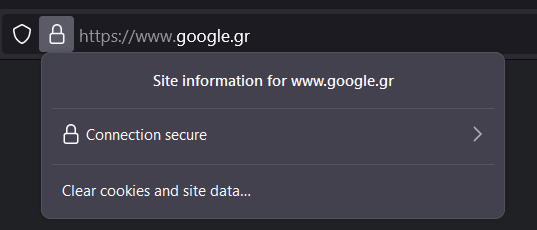
\includegraphics[width=0.8\textwidth]{C:/Users/dimit/Desktop/TeX/EC/google1}
	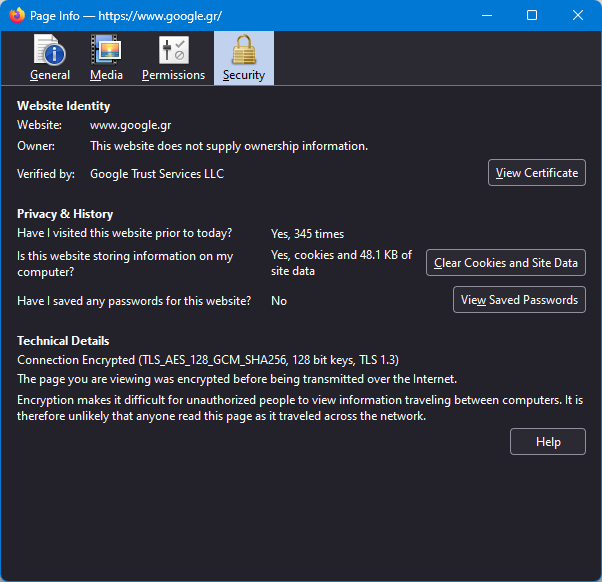
\includegraphics[width=0.8\textwidth]{C:/Users/dimit/Desktop/TeX/EC/google2}
\end{figure}
Θα δούμε ότι χρησιμοποιεί την ακόλουθη καμπύλη με το ακόλουθο δημόσιο κλειδί:
\begin{figure}[H]
	\centering
	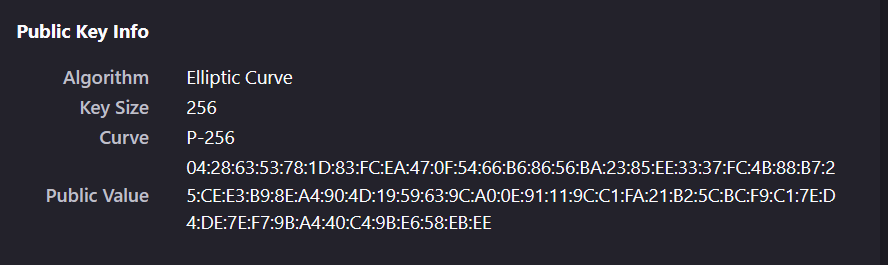
\includegraphics[width=0.8\textwidth]{C:/Users/dimit/Desktop/TeX/EC/google3}
\end{figure}

$ $\newline
Η οποία είναι η $P-256$ από το Εθνικό Ινστιτούτο Προτύπων και Τεχνολογίας (\tl{NIST}) της Αμερικής. Όπως φαίνεται εδώ αλλά και στα παραδείγματα που υπάρχουν έτοιμες οι καμπύλες στις βιβλιοθήκες της \tl{Python}, δεν κάνει κανείς κρυπτογραφία με το να φτιάχνει τις δικές του ελλειπτικές καμπύλες καθώς πρέπει αφενός να αντιστέκονται στις επιθέσεις και αφετέρου να μην υπάρχουν άλλα κενά ασφαλείας. Για την αντοχή στις επιθέσεις, υπάρχουν πολλά πρότυπα για την επιλογή ελλειπτικών καμπυλών που θεωρούνται ασφαλείς όπως τα:
\begin{itemize}
	%safecurves.cr.yp.to να βάλω τα hyperlinks αν είναι
	\item \tl{ANSI X9.62} (1999).
	\item \tl{IEEE P1363} (2000).
	\item \tl{SEC 2} (2000).
	\item \tl{NIST FIPS} 186-2 (2000).
	\item \tl{ANSI X9.63} (2001).
	\item \tl{Brainpool} (2005).
	\item \tl{NSA Suite B} (2005).
	\item \tl{ANSSI FRP256V1} (2011).
\end{itemize}

$ $\newline
Στον σύνδεσμο \tl{www.rfc-editor.org/rfc/rfc5639} είναι δημοσιευμένος ο αλγόριθμος για την επιλογή παραμέτρων των \tl{NIST} και \tl{Brainpool} καμπυλών. Η εύρεση ασφαλών ελλειπτικών καμπυλών είναι κάτι που μελετάται συνεχώς. Η \tl{Certicom} ανανεώνει την λίστα \tl{Standards for Efficient Cryptography: Recommended Elliptic Curve Parameters (SEC 2)} κάθε πέντε χρόνια \cite{sec2} και γίνονται συνεχώς νέες προσπάθειες όπως η πρόσφατη στο \cite{lenstra}.

$ $\newline
Δυστυχώς, υπάρχει ένα χάσμα μεταξύ της δυσκολίας του \tl{ECDLP} και της ασφάλειας του \tl{ECC}. Το \tl{ECDLP} έχει να κάνει με το να ανακτήσει κάποιος το ιδιωτικό κλειδί του \tl{ECC} χρήστη με δεδομένο το δημόσιο κλειδί. Ακόμα και κάποιος να χρησιμοποιεί τις παραπάνω καμπύλες, οι πιθανότητες να τις χρησιμοποιεί θεωρητικά σωστά είναι εναντίων του. Υπάρχουν πολλές πραγματικές επιθέσεις στο \tl{ECC} που δεν χρειάζεται να λύσουν το \tl{ECDLP}. Για παράδειγμα, σε μια υλοποίηση μπορεί να συμβαίνουν τα ακόλουθα:
\begin{itemize}
	\item Να παράγει λάθος αποτέλεσμα για σημεία της καμπύλης που προκύπτουν σπάνια.
	\item Να διαρρέει εσωτερική πληροφορία όταν δωθεί σαν είσοδος κάτι που δεν είναι σημείο στην καμπύλη.
	\item Να δέχεται \tl{timing} επιθέσεις, δηλαδή να εκμεταλλεύεται κάποιος επιτιθέμενος τον χρόνο που χρειάζεται η υλοποίηση να τρέξει τους κρυπτογραφικούς αλγορίθμους και έτσι να διαρρέει εσωτερική πληροφορία.
\end{itemize} 

$ $\newline
Οι επιτιθέμενοι ουσιαστικά εκμεταλλεύονται αυτό το χάσμα του \tl{ECDLP} και του \tl{ECC} για τους ακόλουθους λόγους:
\begin{itemize}
	\item Το \tl{ECDLP} είναι θεωρητικό πρόβλημα, ενώ το \tl{ECC} αντιδρά με τις εισόδους του χρήστη που μπορεί να είναι κακόβουλες.
	\item Το \tl{ECDLP} δίνει μόνο την πληροφορία $nP$, ενώ από το \tl{ECC} μπορεί να ξεφεύγει με διάφορους τρόπους πληροφορία από το κανάλι και από το εσωτερικό σύστημα, καθώς και χρόνοι εκτέλεσης.
	\item Το \tl{ECDLP} απλά υπολογίζει το $nP$ θεωρητικά σωστά, ενώ στην πραγματικότητα στο \tl{ECC} μπορεί να υπάρξουν σφάλματα.
\end{itemize}

$ $\newline
Ένα νέο έργο που προσπαθεί να προσφέρει και \tl{ECC} ασφάλεια πέρα από \tl{ECDLP} είναι το \tl{SafeCurves} των \tl{Daniel Bernstein} και \tl{Tanja Lange} \cite{safecurves}. Το συγκεκριμένο έργο περνάει ένα επιπλέον φιλτράρισμα για \tl{ECC} ασφάλεια στις λίστες των καμπυλών που αναφέρθηκαν προηγουμένως.

\begin{figure}[H]
	\centering
	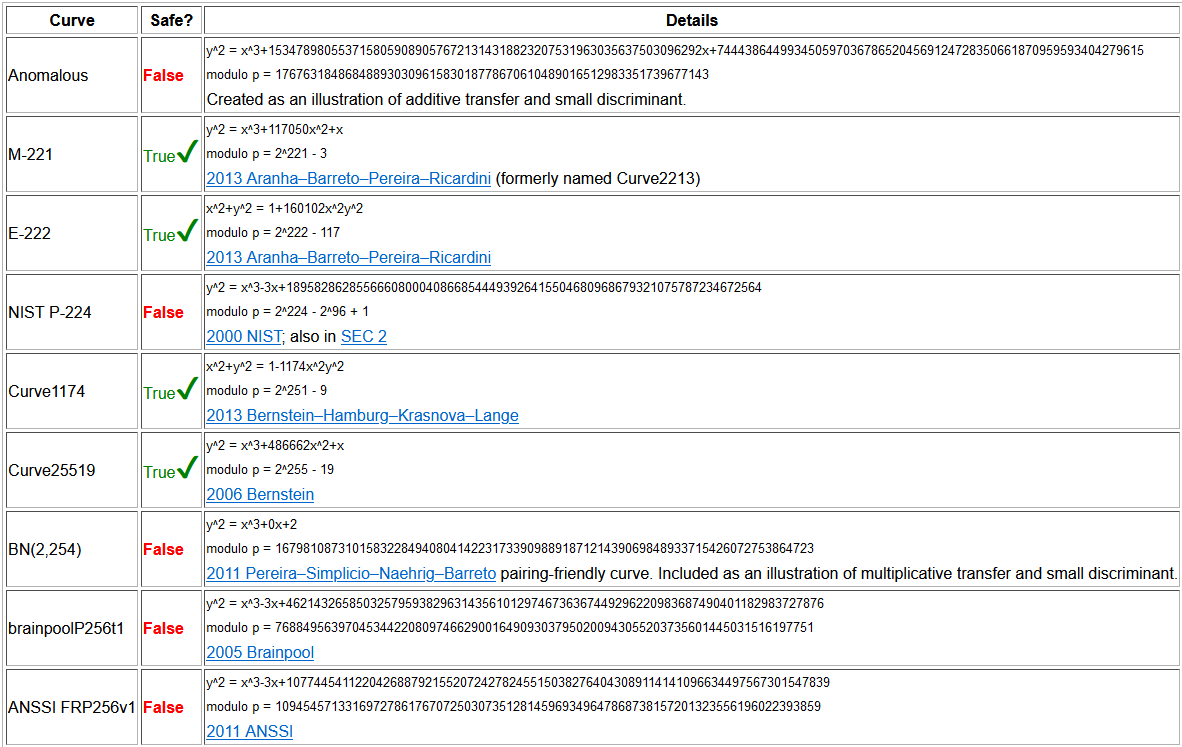
\includegraphics[width=1\textwidth]{C:/Users/dimit/Desktop/TeX/EC/curves1}
	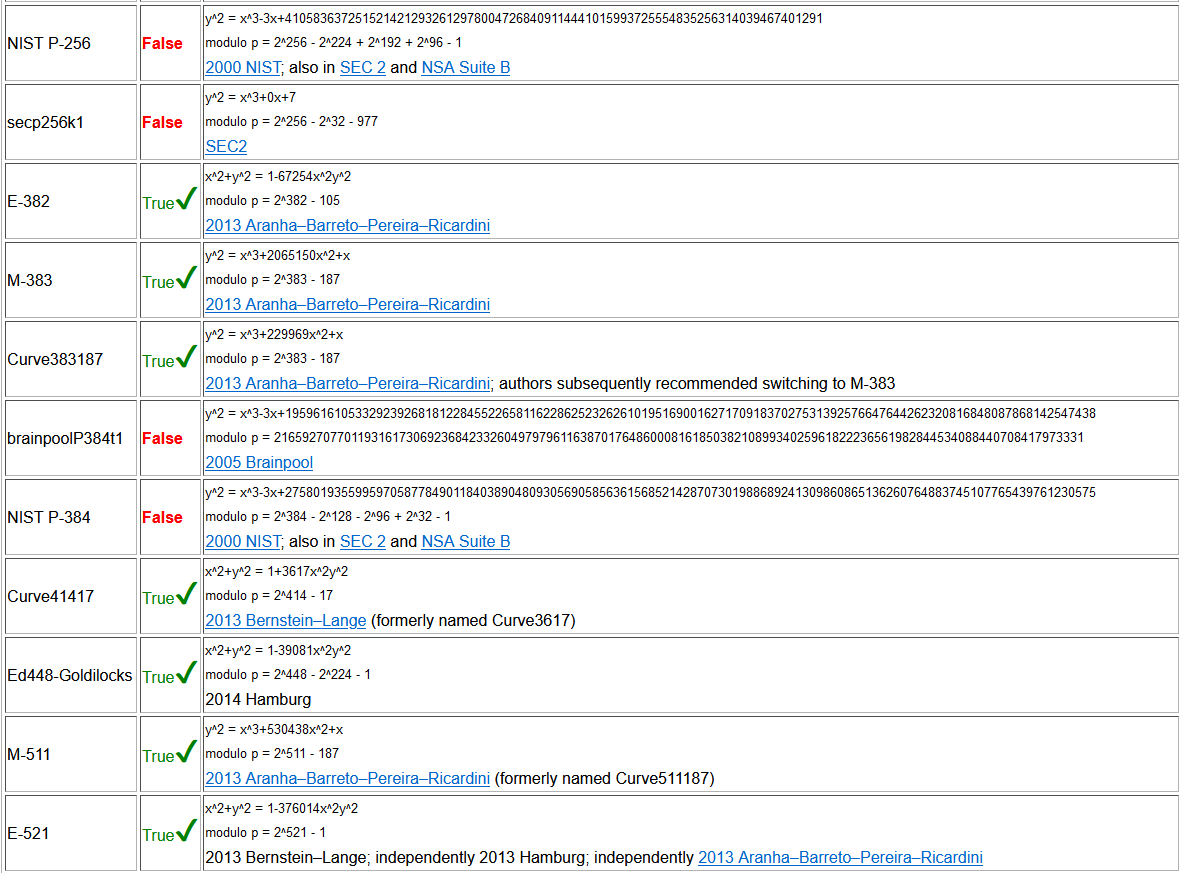
\includegraphics[width=1\textwidth]{C:/Users/dimit/Desktop/TeX/EC/curves2}
\end{figure}
\begin{figure}[H]
	\centering

	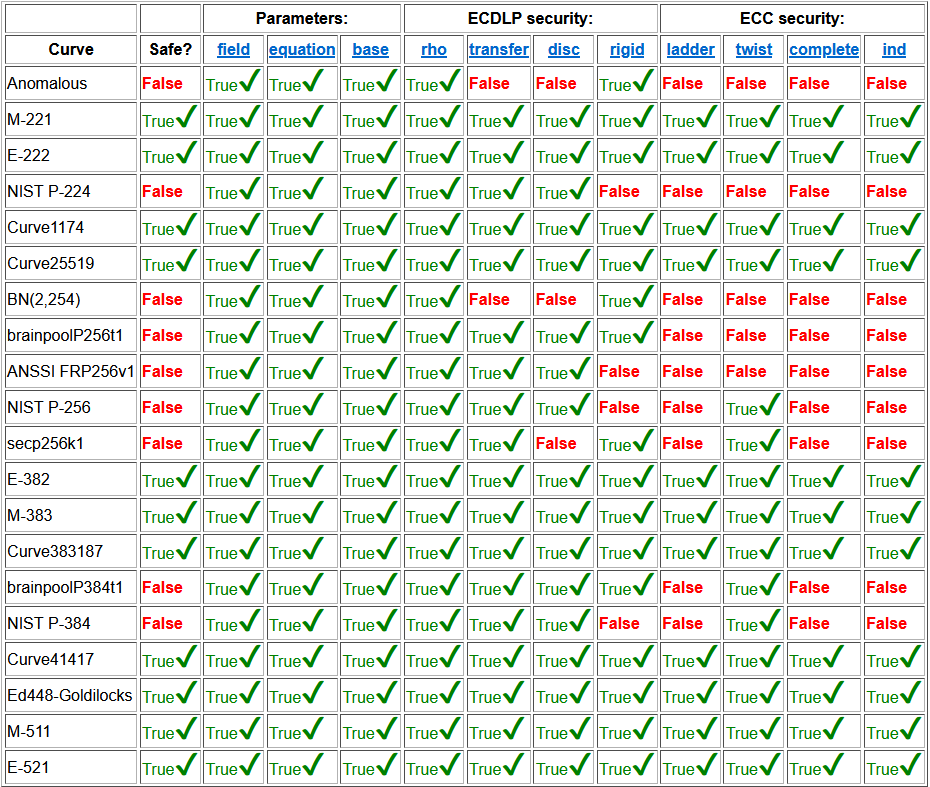
\includegraphics[width=1\textwidth]{C:/Users/dimit/Desktop/TeX/EC/curves3}
	\captionsetup{labelformat=empty}
	\caption{Πίνακες από \tl{SafeCurves} \cite{safecurves}}
\end{figure}

$ $\newline
Όπως βλέπουμε, οι διάσημες ελλειπτικές καμπύλες \tl{NIST P-256} και \tl{secp256k1} δεν θεωρούνται ασφαλείς από τα επιπλέον κριτήρια του \tl{SafeCurves}.

\pagebreak
\section{Περαιτέρω μελέτη και \tl{Isogenies}}

\vspace*{0.3cm}
\noindent Καθώς το πρόβλημα \tl{ECDLP} παραμένει σήμερα υπολογιστικά δύσκολο, στο οποίο βασίζεται και η ανταλλαγή κλειδιού \tl{ECDH}, δεν θα ισχύει το ίδιο στο μέλλον όταν ένας επιτιθέμενος θα μπορεί να χρησιμοποιήσει έναν μεγάλης κλίμακας κβαντικό υπολογιστή. Ο μαθηματικός \tl{Peter Shor} έδειξε με δικό του αλγόριθμο \cite{shor} ότι ένας κβαντικός υπολογιστής που καταφέρνει να λειτουργεί ορθά με αρκετά \tl{q-bits} μπορεί να σπάσει σε πολυωνυμικό χρόνο τα ακόλουθα:
\begin{itemize}
	\item Το σχήμα \tl{RSA}.
	\item Το πρωτόκολλο ανταλλαγής κλειδιού \tl{Diffie-Hellman} σε πεπερασμένα σώματα.
	\item Το πρωτόκολλο ανταλλαγής κλειδιού \tl{ECDH}.
\end{itemize} 

$ $\newline
Μέχρι να υπάρξει ένας τέτοιος υπολογιστής, καλούνται οι μαθηματικοί να έχουν έτοιμους κρυπτογραφικούς αλγορίθμους που αποδεδειγμένα να έχουν αντοχή ενάντια σε επιθέσεις που χρησιμοποιούν συγκεκριμένο πλήθος \tl{q-bits}. Ένας τέτοιος μετα-κβαντικός αλγόριθμος είναι ο \tl{Supersingular Isogeny-Based Diffie-Hellman (SIDH)} που βασίζεται σε \tl{isogenies} και \tl{supersingular} ελλειπτικές καμπύλες. Η ιδέα είναι ότι θέλουμε ένα πρωτόκολλο σαν το \tl{ECDH} που να είναι ασφαλές από κβαντικούς υπολογιστές. Σκεφτόμαστε τον βαθμωτό πολλαπλασιασμό:
$$n P  = P + P + \cdots + P$$ σαν μια απεικόνιση μεταξύ της ελλειπτικής καμπύλης $E$:

$$ E \longrightarrow E$$
$$ P \longmapsto n P$$

$ $\newline
Ουσιαστικά θέλουμε να έχουμε γενικότερες απεικονίσεις που απεικονίζουν ελλειπτικές καμπύλες σε ελλειπτικές καμπύλες. Επιπλέον, αντίθετα από τον βαθμωτό πολλαπλασιασμό, δεν χρειάζεται αυτές οι απεικονίσεις να ξεκινούν και να τελειώνουν στην ίδια καμπύλη $E$. 

\vspace*{0.1cm}
\begin{defn}[Ρητή Απεικόνιση]
	Μια ρητή απεικόνιση μεταξύ ελλειπτικών καμπύλων είναι μια απεικόνιση που η κάθε συντεταγμένη είναι ο λόγος πολυωνύμων. Δηλαδή:
	$$\Phi(P) = \phi(x,y) = \left(\frac{p_1(x,y)}{q_1(x,y)}, \frac{p_2(x,y)}{q_2(x,y)}\right)$$ με $p_1,p_2,q_1,q_2$ πολυώνυμα δύο μεταβλητών πάνω από το σώμα που ορίζεται η ελλειπτική καμπύλη.
\end{defn}

$ $\newline
Καθώς ο πολλαπλασιασμός διατηρεί την πρόσθεση, δηλαδή:
$$n(P+Q) = nP + nQ$$ θέλουμε να συμβαίνει το αντίστοιχο:
$$\Phi(P+Q) = \Phi(P) + \Phi(Q)$$ δηλαδή η $\Phi$ να είναι ομομορφισμός ομάδων. Έτσι καταλήγουμε στον ορισμό:

\vspace*{0.3cm}
\begin{defn}[\tl{Isogeny}]
	Ένα \tl{isogeny} μεταξύ δύο ελλειπτικών καμπυλών $E_1,E_2$ είναι μια ρητή απεικόνιση $\Phi: E_1 \rightarrow E_2$ που είναι ομομορφισμός ομάδων.
\end{defn}

$ $\newline
Η ιδέα τώρα είναι πιο ξεκάθαρη, αν δούμε σε αντιστοιχία το \tl{ECDH} με το \tl{SIDH} αντίστοιχα:
\vspace*{0.3cm}
\begin{figure}[H]
	\centering
	\begin{tikzcd}
		A:                                       &  & n_A P \arrow[rdd, dashed] & n_B P \arrow[rrd, "n_A"]  &  &               \\
		P \arrow[rru, "n_A"] \arrow[rrd, "n_B"'] &  &                           &                           &  & S = n_A n_B P \\
		B:                                       &  & n_B P \arrow[ruu, dashed] & n_A P \arrow[rru, "n_B"'] &  &              
		\end{tikzcd}
\end{figure}


\begin{figure}[H]
	\centering
\begin{tikzcd}
	A:                                             &  & E_A \arrow[rdd, dashed] & E_B \arrow[rrd, "\Psi_A"] &  &                      \\
	E \arrow[rru, "\Phi_A"] \arrow[rrd, "\Phi_B"'] &  &                         &                           &  & E_{AB} \simeq E_{BA} \\
	B:                                             &  & E_B \arrow[ruu, dashed] & E_A \arrow[rru, "n_B"']   &  &                     
	\end{tikzcd}
\end{figure}

$ $\newline
Δηλαδή, θέλουμε να αντικατασταθούν τα ιδιωτικά κλειδιά $n_A, n_B$ από τα \tl{isogenies} $\Phi_A, \Phi_B$. Τα $\Psi_A, \Psi_B$ είναι στην ουσία το ίδια με τα $\Phi_A, \Phi_B$ αντίστοιχα, απλά ξεκινούν από διαφορετική καμπύλη. Όπως σε αντιστοιχία ο δεύτερος πολλαπλασιασμός με $n_A$ δεν ξεκινάει από το $P$ αλλά από το $n_B P$.  Ουσιαστικά, το ιδιωτικό κλειδί της \tl{Alice} θα είναι το $\Phi_A$ με το οποίο θα μπορεί να βρει το $\Psi_A$ και όμοια θα γίνεται η ίδια διαδικασία για τον \tl{Bob}.

$ $\newline
Στο \tl{ECDH} τα δημόσια κλειδία είναι η εικόνα ενός σημείου μέσα από την απεικόνιση πολλαπλασιασμού. Εδώ στο \tl{SIDH} η διαφορά είναι ότι πλέον το δημόσιο κλειδί δεν θα είναι ένα σημείο, αλλά όπως φαίνεται στο παραπάνω διάγραμμα, θα είναι ολόκληρη η καμπύλη εικόνα. Αυτό βασίζεται στην πρόταση:

\vspace*{0.1cm}
\begin{prop}
	Αν έχουμε \tl{isogeny} $\Phi:E \rightarrow E^{\prime}$ τότε η εικόνα $\Phi(E)$ είναι ελλειπτική καμπύλη. Οπότε πλέον θεωρούμε τα \tl{isogenies} να είναι επιμορφισμοί ομάδων.
\end{prop}

$ $\newline
Οπότε το δημόσιο κλειδί της \tl{Alice} θα είναι το $E_A = \Phi_A(E)$. Για τεχνικούς λόγους, θα περιλαμβάνονται όπως θα δούμε στο δημόσιο κλειδία και δύο επιπλέον σημεία.

$ $\newline
Για το κοινό μυστικό, στο \tl{ECDH} υπολογίζεται ακριβώς το ίδιο σημείο $n_A n_B P$. Δυστυχώς, στο \tl{SIDH} οι αντίστοιχες εικόνες $E_{AB}$ και $E_{BA}$ δεν είναι απαραίτητα η ίδια καμπύλη. Ωστόσο, έχουν την ίδια δομή με βάση τα ακόλουθα:

\vspace*{0.1cm}
\begin{defn}[Ισομορφισμός] Θα λέμε ισομορφισμό ελλειπτικών καμπυλών $E_1,E_2$ ένα \tl{isogeny} μεταξύ τους που είναι 1-1, δηλαδή μονομορφισμός ομάδων. Δύο ελλειπτικές καμπύλες θα είναι ισόμορφες αν υπάρχει τέτοιο \tl{isogeny} μεταξύ τους.
\end{defn}

$ $\newline
Ένα χρήσιμο κριτήριο για τον ισομορφισμό είναι με βάση ένα αναλλοίωτο μέγεθος που έχουν οι ελλειπτικές καμπύλες.
\vspace*{0.1cm}
\begin{defn}[$j$-\tl{invariant}]
	Έστω ελλειπτική καμπύλη $E: y^2 = x^3 + ax + b$, ορίζουμε ως $j$-\tl{invariant} της $E$ το μέγεθος:
	$$j(E) = \frac{6912 a^3}{4a^3 + 27b^2}$$
\end{defn}
\vspace*{0.1cm}
\begin{prop} Δύο ελλειπτικές καμπύλες είναι ισόμορφες (πάνω από την αλγεβρική θήκη του ίδιου σώματος) αν και μόνο αν έχουν το ίδιο $j$-\tl{invariant}.
\end{prop}

$ $\newline
Οπότε για την περίπτωση του \tl{SIDH}, έχουμε ότι οι καμπύλες $E_{AB}, E_{BA}$ δεν είναι απαραίτητα ίδιες, αλλά ισχύουν τα:
$$E_{AB} \simeq E_{BA}$$
$$j(E_{AB}) = j(E_{BA})$$

$ $\newline
Άρα πρέπει η \tl{Alice} και ο \tl{Bob} να έχουν έναν τρόπο να διαλέγουν τυχαία \tl{isogenies}. Αυτό γίνεται εύχρηστα στην κρυπτογραφία βασισμένη σε \tl{isogenies} με τον ορισμό του πυρήνα:

\vspace*{0.1cm}
\begin{defn}[Πυρήνας \tl{Isogeny}]
	Έστω $\Phi : E_1 \longrightarrow E_2$ \tl{isogeny}, ο πυρήνας που συμβολίζεται $\ker \Phi$ είναι το σύνολο των στοιχείων:
	$$\ker \Phi = \{P \in E_1 | \quad \Phi(P) = \mathcal{O}\}$$
\end{defn}

$ $\newline
Με την ακόλουθη πρόταση παίρνουμε έναν τρόπο να ορίζουμε ολόκληρα \tl{isogenies} μόνο ορίζοντας τον πυρήνα τους:
\vspace*{0.1cm}
\begin{prop}
	Αν δύο \tl{isogenies} έχουν τον ίδιο πυρήνα, τότε οι ελλειπτικές καμπύλες εικόνες τους είναι ισόμορφες.
\end{prop}

$ $\newline
Και μπορούμε να ορίσουμε πυρήνες εύκολα ως την γραμμική θήκη στοιχείων, δηλαδή:
$$\langle P_1,P_2,\ldots,P_n \rangle = \{m_1 P_1 + m_2 P_2 +\cdots + m_n P_n \in E| \quad m_i \in \mathbb{Z}\}$$ και ένα \tl{isogeny} που ορίζεται από πυρήνα $\langle P \rangle$, δηλαδή από ένα στοιχείο θα λέγεται κυκλικό \tl{isogeny}. 

$ $\newline
Οπότε, για να δημιουργήσει το ζεύγος κλειδιών της η \tl{Alice} πρέπει να επιλέξει τυχαία ένα σημείο $R_A$ της ελλειπτικής καμπύλης συγκεκριμένης τάξης και με αυτό να έχει τον πυρήνα $\langle R_A \rangle$ και το \tl{isogeny} $\Phi_A$ που ορίζει αυτό ως ιδιωτικό κλειδί. Στην συνέχεια, παίρνει το δημόσιο κλειδί της $E_A = \Phi_A(E)$. Δηλαδή, το πρόβλημα μεταφέρεται στο να μπορεί να επιλέξει τυχαία το σημείο $R_A$ στην καμπύλη.

$ $\newline
Συνήθως, στην κρυπτογραφία βασισμένη σε \tl{isogenies} γίνονται οι πράξεις σε μια ελλειπτική καμπύλη $E$ πάνω από το $\mathbb{F}_{p^2}$ για κάποιον πρώτο της μορφής $p=2^a 3^b -1$ με $a,b \in \mathbb{N}$. Χρησιμοποιείται επιπλέον ότι οι υποομάδες στρέψης $E[2^a]$ και $E[3^b]$ μπορούν να παραχθούν από δύο στοιχεία το καθένα $P_A,Q_A$ και $P_B,Q_B$ αντίστοιχα. Έτσι, αυτά τα δύο σημεία (για τα οποία υπάρχουν πολλές επιλογές σαν βάση) θα είναι η επιπλέον πληροφορία που θα περιλαμβάνει το δημόσιο κλειδί. Έτσι, η \tl{Alice} μπορεί πλέον να επιλέξει τυχαία με τους ήδη γνωστούς τρόπους έναν φυσικό αριθμό $r_A$ και αυτό να της δώσει το αντίστοιχο σημείο $R_A$ ως εξής:
$$0\leq r_A \leq 2^a$$
$$R_A = P_A + r_A Q_A$$

$ $\newline
και η υποομάδα $\langle R_A \rangle$ βρίσκεται μέσα στην υποομάδα στρέψης $E[2^a]$. Αντίστοιχα, ο \tl{Bob} θα έχει ένα \tl{isogeny} με πυρήνα $\langle R_B \rangle$ που βρίσκεται μέσα στην $E[3^b]$. Το ότι οι τάξεις των πυρήνων των \tl{isogenies} είναι δυνάμεις μικρών πρώτων αριθμών κάνει πιο γρήγορο τον υπολογισμό τους, καθώς και είναι βοηθητικό οι τάξεις να είναι σχετικά πρώτες. Τα μεγέθη $a,b$ συσχετίζονται με την ασφάλεια που έχει το πρωτόκολλο.


$ $\newline
Θέλουμε να καταλήξουμε σε ίδια $j$-\tl{invariants} και αυτό πετυχαίνεται με το να ορίσουμε $\Psi_A$ το \tl{isogeny} που προκύπτει από τον πυρήνα $\langle \Phi_B(R_A) \rangle$. Αποδεικνέται ότι:
$$\Psi_A \circ \Phi_B = \langle R_A, R_B \rangle$$ και όμοια:
$$\Psi_B \circ \Phi_A = \langle R_A, R_B \rangle$$ έτσι θα έχουμε:
$$\ker (\Psi_A \circ \Phi_B) = \ker (\Psi_B \circ \Phi_A)$$ και άρα αποδεικνέται ότι:
$$E_{AB} = \Psi_A \circ \Phi_B(E) \simeq \Psi_B \circ \Phi_A (E) = E_{BA}$$ Συνεπώς, η \tl{Alice} και ο \tl{Bob} παίρνουν ως κοινό μυστικό την τιμή:
$$j(E_{AB}) = j(E_{BA})$$

$ $\newline
Όπως φαίνεται παραπάνω, για να κατασκευάσει η \tl{Alice} το $\Psi_A$ χρειάζεται να ξέρει το $\Phi_B(R_A)$. Για αυτόν τον λόγο, ο \tl{Bob} στο δημόσιο κλειδί του περιλαμβάνει τις τιμές $$\Phi_B(P_A), \Phi_B(Q_A)$$, δηλαδή τις εικόνες της προκαθορισμένης βάσης του $E[2^a]$ μέσω της $\Phi_B$ που είναι το ιδιωτικό κλειδί του \tl{Bob}. Έτσι, η \tl{Alice} μπορεί να υπολογίσει:
$$\Phi_B(R_A) =  \Phi_B(P_A) + r_A \Phi_B(Q_A)$$

$ $\newline
Συνδυάζοντας τα παραπάνω, μπορούμε να κάνουμε το διάγραμμα του πρωτοκόλλου \tl{SIDH}. Χρειαζόμαστε μια καμπύλη $E$ που αντέχει μια κβαντική επίθεση όπως αυτή του \tl{Shor} που σπάει το \tl{ECDH}. Συγκεκριμένα, μπορούμε να διαλέξουμε $E: y^2 = x^3 +ax+b$ πάνω από το $\mathbb{F}_{p^2}$ για πρώτο $p=2^a 3^b -1$, αλλά και οποιαδήποτε \tl{supersingular} καμπύλη αρκεί. \tl{Supersingular} είναι οι καμπύλες πάνω από το σώμα $K$ για τις οποίες ισχύει το παρακάτω για τις υποομάδες στρέψης:
$$E[p^r](K) = \begin{cases}
	\mathbb{Z}/p^r \mathbb{Z} & \text{ ή }\\
	0
\end{cases}$$ 

$ $\newline
Οπότε, έχοντας τις ακόλουθες δημόσιες παραμέτρους:
$$E(\mathbb{F}_{p^2}): \quad y^2=x^3+ax+b$$
$$p = 2^a 3^b -1, \quad a,b \in \mathbb{N}$$
$$P_A, Q_A \ \text{ μια βάση του } \ E[2^a]$$
$$P_B, Q_B \ \text{ μια βάση του } \ E[3^b]$$

$ $\newline
Έχουμε στην επόμενη σελίδα το διάγραμμα του πρωτοκόλλου ανταλλαγής κλειδιού \tl{SIDH}:


\procedureblock{\tl{SIDH}}{
	\textbf{\tl{Alice}} \> \> \textbf{\tl{Bob}} \\
	\text{Διάλεξε } 0\leq r_A <2^a \> \> \text{Διάλεξε } 0\leq r_B <3^b\\
	r_A \text{ ιδιωτικό κλειδί} \> \> r_B \text{ ιδιωτικό κλειδί} \\ 
	\> \> \\
	\text{Δημόσιο κλειδί: } \> \>  \text{Δημόσιο κλειδί: }\\
	E_A = \Phi_A(E),\Phi_A(P_B), \Phi_A(Q_B) \> \> E_B = \Phi_B(E),\Phi_B(P_A), \Phi_B(Q_A) \\
	\text{όπου } \Phi_A \text{ \tl{isogeny} με }  \> \> \text{όπου } \Phi_B \text{ \tl{isogeny} με } \\ 
	\ker \Phi_A = \langle P_A + r_A Q_A \rangle \> \> \ker \Phi_B = \langle P_B + r_B Q_B \rangle \\
	\> \sendmessageright*{\text{ στέλνει η \tl{Alice} το } E_A} \> \\
	\> \sendmessageleft*{\text{ στέλνει ο \tl{Bob} το } E_B} \> \\
	\text{Κοινό μυστικό: } \> \> \text{Κοινό μυστικό: }\\
	j(\Psi_A(E_B)) \> \> j(\Psi_B(E_A)) \\
	\text{όπου } \Psi_A \text{ \tl{isogeny} με } \>\> \text{όπου } \Psi_B \text{ \tl{isogeny} με }\\
	\ker \Psi_A = \langle \Phi_B(P_A) + r_A \Phi_B(Q_A)\rangle \> \> \ker \Psi_B = \langle \Phi_A(P_B) + r_B \Phi_A(Q_B)\rangle \\
	\> \> \\
	\text{Κλειδί:} \> j(\Psi_A(E_B)) = j(\Psi_B(E_A)) \> 
}

$ $\newline
Εν κατακλείδι, η ασφάλεια του \tl{SIDH} οφείλεται στην δυσκολία του ακόλουθου προβλήματος:
\vspace*{0.3cm}
\begin{defn}
	Υποθέτουμε ότι υπάρχει \tl{isogeny} $\Phi$ μεταξύ δύο ελλειπτικών καμπύλων $E_1, E_2$, όπου ο πυρήνας έχει τάξη $\ell^e$. Το $\ell^e$-\tl{isogeny} πρόβλημα είναι το πρόβημα του να υπολογίσει κανείς τον πυρήνα $\ker \Phi$ δεδομένου μόνο των $E_1, E_2$.
\end{defn}
\vspace*{0.5cm}

$ $\newline
Δηλαδή, πρέπει τα αντίστοιχα $2^a,3^b$-\tl{isogeny} προβλήματα να έιναι δύσκολα, για να μην μπορεί κανείς να βρει το ιδιωτικό κλειδί της \tl{Alice} ή του \tl{Bob} αντίστοιχα. Αυτό το πρόβλημα έχει μελετηθεί τα τελευταία 20 χρόνια από μαθηματικούς που ειδικεύονται στην θεωρία αριθμών και θεωρείται εξαιρετικά δύσκολο για μεγάλες δυνάμεις του $\ell$, για οποιονδήποτε φυσικό αριθμό $\ell$. Συνεπώς, θεωρείται ότι είναι ικανό να αντέξει επίθεση από κβαντικό υπολογιστή μεγάλης κλίμακας και για αυτό είναι πλέον υποψήφιο πρωτόκολλο από το \tl{NIST} για διάφορες κρυπτογραφικές διαδικασίες στην μετα-κβαντική κρυπτογραφία \cite{nistquantum}.


\pagebreak
\section{Βιβλιογραφία}
\vspace*{0.5cm}
\begingroup
\renewcommand{\section}[2]{}%
\begin{thebibliography}{}


	\bibitem{akontogar}
	Kontogeorgis, A., \& Antoniadis, I. (2015). Finite Fields and Cryptography [Undergraduate textbook]. Kallipos, Open Academic Editions. http://hdl.handle.net/11419/155 

	\bibitem{wstein}
	W. Stein, 2008. Elementary Number Theory: Primes, Congruences, and Secrets: A Computational Approach. Undergraduate Texts in Mathematics. Springer New York. https://books.google.gr/books?id=5hYd0yX4mrMC.

	\bibitem{sage}
	SageMath, the Sage Mathematics Software System (Version 9.0.0), The Sage Developers, 2022, https://www.sagemath.org.

	\bibitem{python}
	Python Software Foundation. Python Language Reference, version 3.10. Available at http://www.python.org.

	\bibitem{cryptobook}
	S. Nakov, 2018, Practical Cryptography for Developers, Software University, https://cryptobook.nakov.com/.

	\bibitem{pohlig}
	S. Pohlig, M. Hellman, An improved algorithm for computing logarithms over GF(p) and its cryptographic significance, 1977. http://www.ee.stanford.edu/~hellman/publications/28.pdf

	\bibitem{silverman}
	J. H. Silverman, The Arithmetic of Elliptic Curves, Springer-Verlag, 1986.

	\bibitem{washington}
	L. C. Washington, Elliptic Curves: Number Theory and Cryptography, 2008.

	\bibitem{novotney}
	P. Novotney, Weak Curves In Elliptic Curve Cryptography, 2010. https://wstein.org/edu/2010/414/projects/novotney.pdf


	\bibitem{sec1}
	Standards for Efficient Cryptography Group. SEC 1: Elliptic Curve Cryptography, Mar. 2009. Version 2.0. http://www.secg.org/sec1-v2.pdf.

	\bibitem{sec2}
	Standards for Efficient Cryptography Group. SEC 2: Recommended Elliptic Curve Domain Parameters, Jan. 2010. Version 2.0. http://www.secg.org/sec2-v2.pdf.

	\bibitem{shor}
	P. W. Shor. Polynomial-time algorithms for prime factorization and discrete logarithms on a quantum computer. SIAM J. Computing, 26(5):1484–1509, 1997.
	
	\bibitem{phlixos}
	Χ. Πηλιχός, Κρυπτοσυστήματα και Αποδείξεις Μηδενικής Γνώσης στη Μεταθετική και Μη-Μεταθετική Κρυπτογραφία, 2018, Διπλωματική Εργασία.
	
	\bibitem{nist}
	National Institute of Standards and Technology. Recommended Elliptic Curves for Federal Government Use, Jul. 1999. csrc.nist.gov/encryption.

	\bibitem{nistquantum}
	David Jao et al. Supersingular isogeny key encapsulation. NIST Round 1 Submissions for Post-Quantum Cryptography Standardization, November 30, 2017.

	\bibitem{isara}
	ISARA Corporation, Isogeny-Based Cryptography Tutorial, August 1, 2019,  https://www.isara.com/downloads/crypto\_tutorials/Intro-to-Iso-v3.pdf.

	\bibitem{semaev}
	A. Semaev, Evaluation of Discrete Logarithms in a Group of $p$-Torsion Points of an Elliptic Curve in Characteristic $p$, Mathematics of Computation, Volume 67, Number 221, January 1998, Pages 353–356, S 0025-5718(98)00887-4.

	\bibitem{mov}
	A. J. Menezes, T. Okamoto, S. A. Vanstone, Reducing elliptic curve logarithms to a finite field, IEEE Trans., Info Theory, 39 (1993), pp.1639—1646

	\bibitem{safecurves}
	D. J. Bernstein and T. Lange. SafeCurves: choosing safe curves for elliptic-curve cryptography. https://safecurves.cr.yp.to, accessed 1 August 2022. 

	\bibitem{lenstra}
	A. Miele, A. K. Lenstra, Efficient ephemeral elliptic curve cryptographic keys, 2015.
\end{thebibliography}
\endgroup


%ανακτηση δημοσιου κλειδιου http://www.secg.org/sec1-v2.pdf
\end{document}

%αν χρειαστεί extra content γράφω για edwards curves

%να βγάλω το language=Python!!!!
%εκεί που δεν βοηθάει